\section{Analysis}

%Analysis may involve: Interpretation, Presentation, comparison and confirmation

% The analysis chapter will present and discuss the main findings and outcomes, with limits being acknowledged (ie. Survey response levels, generalisability of results, reliability of tests, factos outwith your control.)

\subsection{Data analysis}

% Outline key variables and hypostheses being tested. 
The accuracy, precision, recall and numbers of probes sent will be used as the basis of establishing performance of the contemporary methods. This data is quantitative, with accuracy, precision and recall being continuous and number of probes sent discrete. 

Furthermore, side by side visual comparison between the simulated network topology and the measured network topology will also be presented. This data is categorical and is also binary, due to the compared topologies either being equivalent or not. 

% Data collection
The data will be collected through experimentation in a virtual network lab, as outlined above. Measurement of each configuration will be repeated five times, in order to ensure the validity of the results and allow for statistical analysis. 

% Data preparation
The network topology structure is pre-defined inside a YAML configuration file. Whereby the topology is defined in a set of \textit{nodes} and the \textit{links} between given nodes. Each node has a given \textit{kind} and \textit{image}, with the kind defining the node configuration and behaviour. Each node also has an \textit{image}, which defines the operating system which is to be ran on a given node. Each \textit{link} is defined through an array of end-points between each node. 

% Tools/Mathimatical models used for analysis
Experimental data will be exported in JSON format, from which it can be easily processed. The mean, mode, median and standard deviation will be presented for each finding. Analysis of the implemented model will be carried out using several metrics in order to illustrate comparisons between it's performance and the original model's performance. Several plot types such as scatter plots, line plots and violin plots will be used to visualize; negative and positive correlations and also to represent the standard deviation of results respectively. Furthermore, tables of data will also be used to provide accurate numerical data in a straightforward manner.

% 6. Connect methods to research objectives

%focusing on the study, hypothesis, sample groups you wish to address, and the limitations you have faced.

\subsection{Results}


\subsubsection{Topology set 1}
As shown from the comparison between the shortest path length distribution of Erdos-Renyi, Barabasi-Albert, and real-world topologies, Dataxchange and Layer42; the Erods-Renyi graph with p=0.5 has most closely matches the distribution of shortest path lengths to the real-world topology Dataxchange. With both topologies having frequencies of approximately 0.5 and 0.6 of shortest path length 1.0 respectively. However, there is still some disparity between the frequency of higher shortest path length values between the two topologies. Additionally, the Erdos-Renyi graph with p=0.5 also most closely matches the Layer42 network, with the difference between the shortest path length value 1.0 being approximately 1 and approximately 0.75 for shortest path length value 2.0.  

\begin{figure}
    \centering
    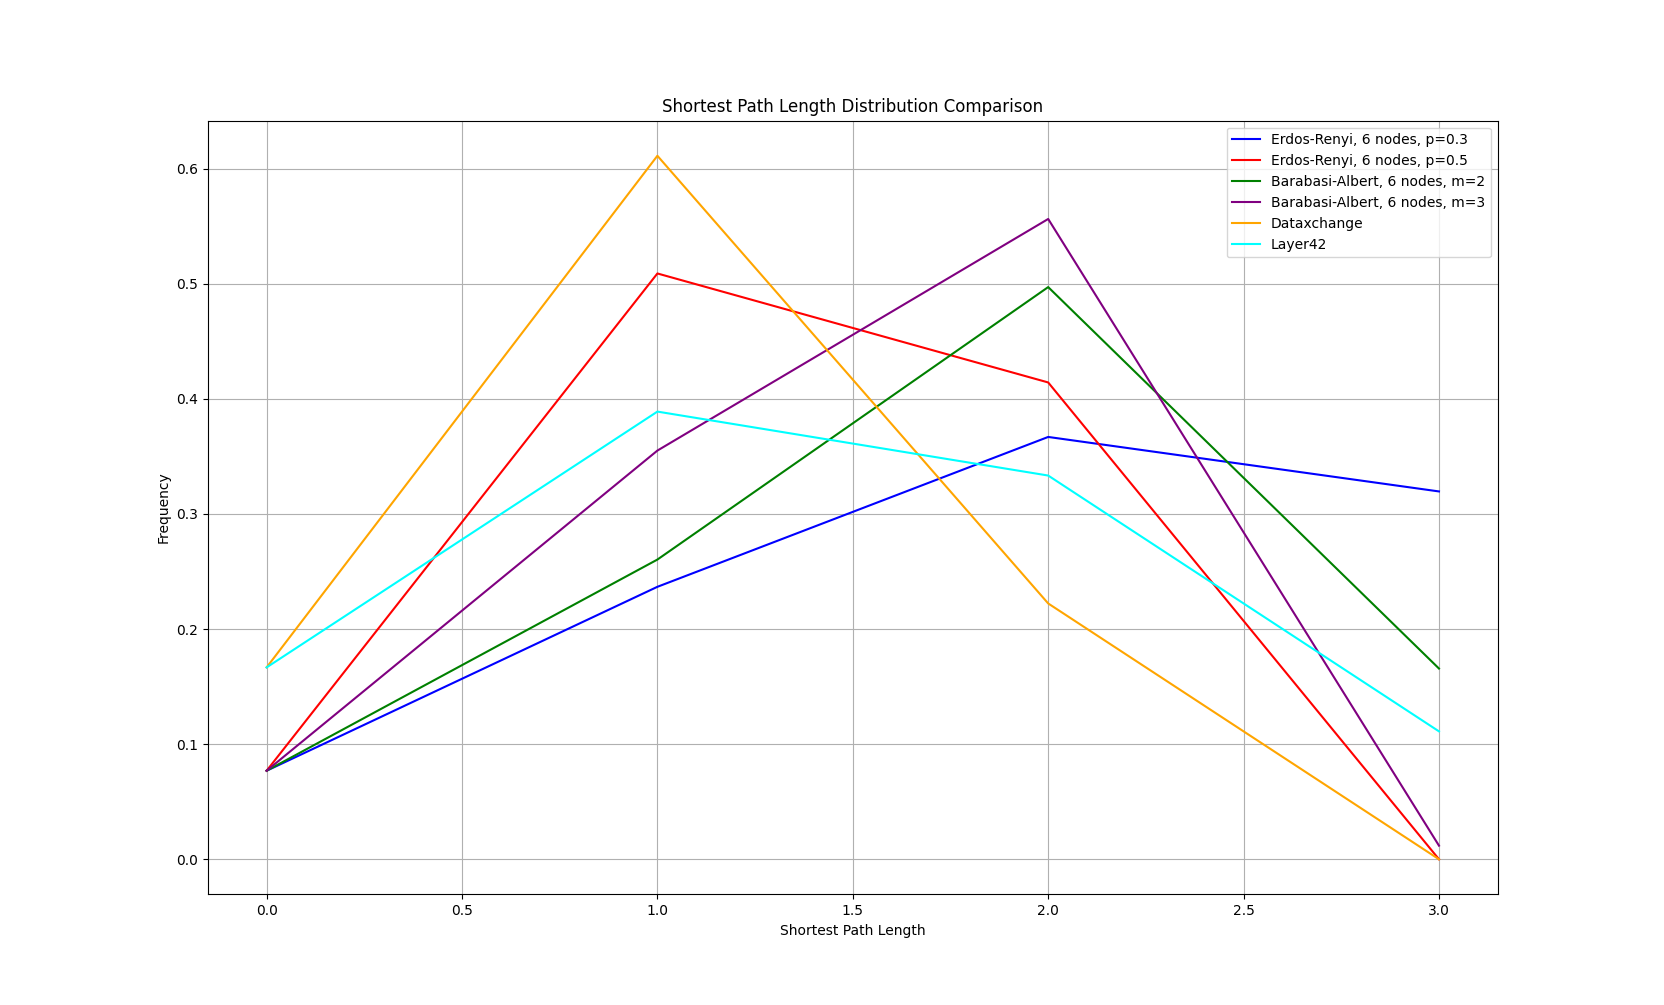
\includegraphics[width=0.9\linewidth]{images/FINAL-TOPO-COMP/line-6.png}
    \caption{Caption}
    \label{fig:enter-label}
\end{figure}

\begin{figure}
    \centering
    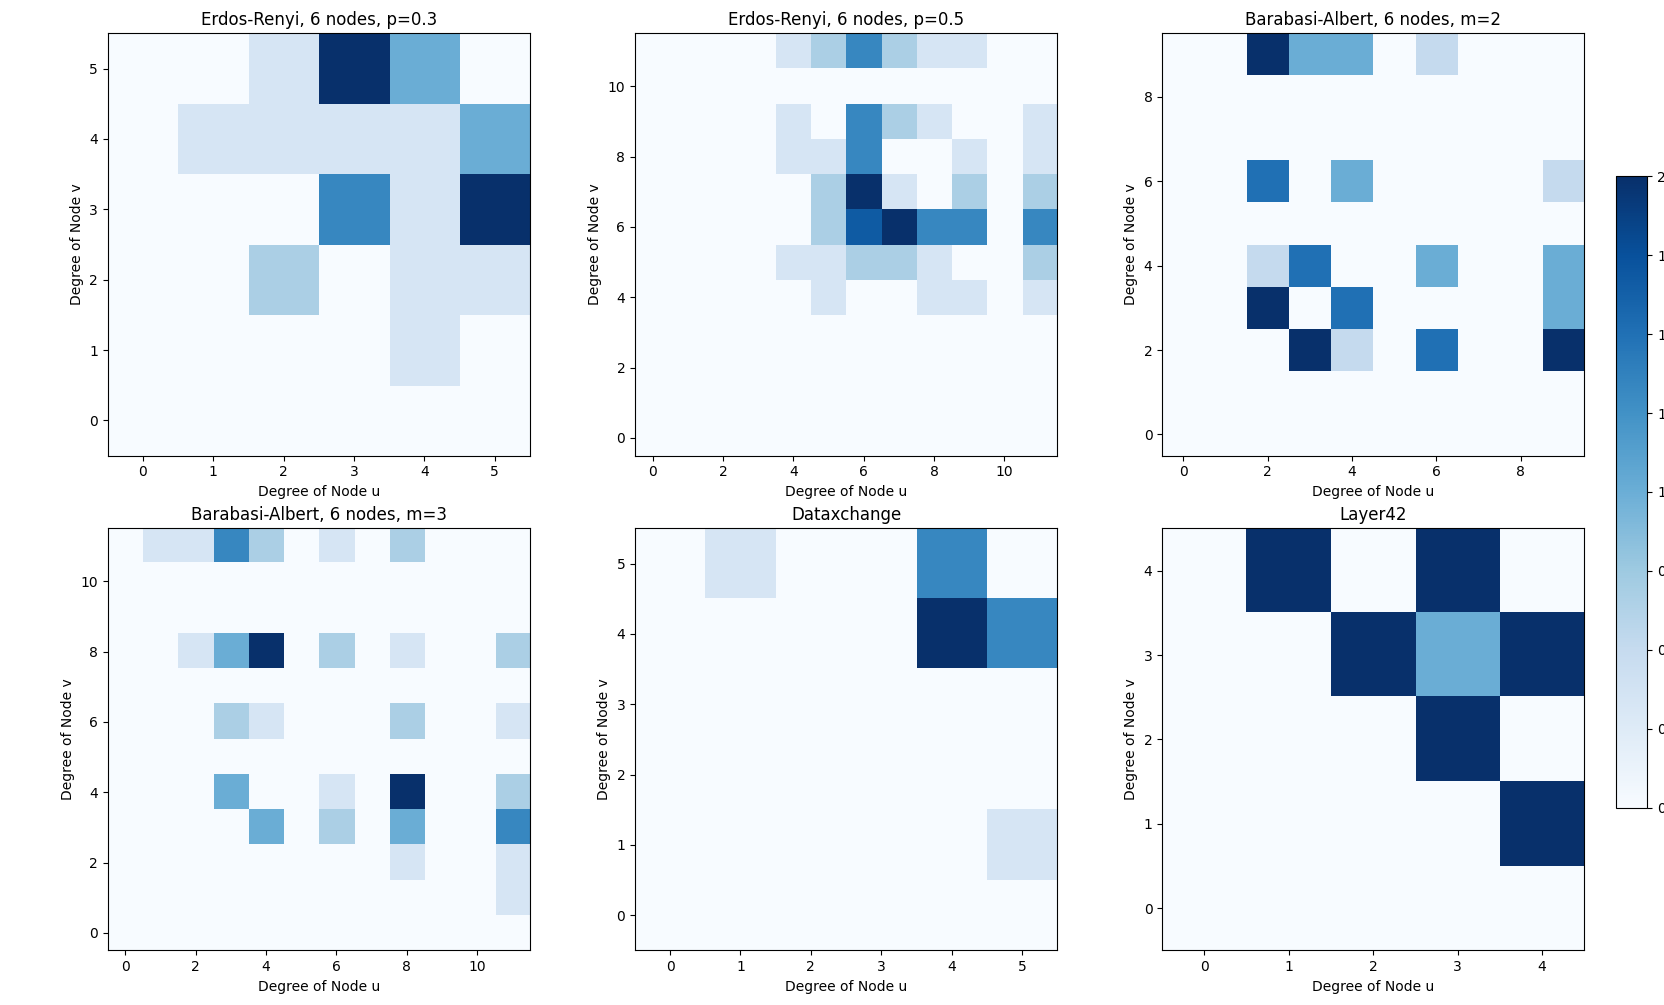
\includegraphics[width=0.9\linewidth]{images/FINAL-TOPO-COMP/Degree-correlation-matrices/6-matrix.png}
    \caption{Caption}
    \label{fig:enter-label}
\end{figure}

However, when taking into consideration the degree correlation coefficient, the Barabasi-Albert graph with m=3, is the most closely correlated to both the Dataxchange and Layer42 networks. The Barabasi-Albert generated network has an $r$ value of -0.49, compared with $r$ values of -0.45 and -0.6 for Dataxchange and Layer42 respectively.  

\begin{figure}
    \centering
    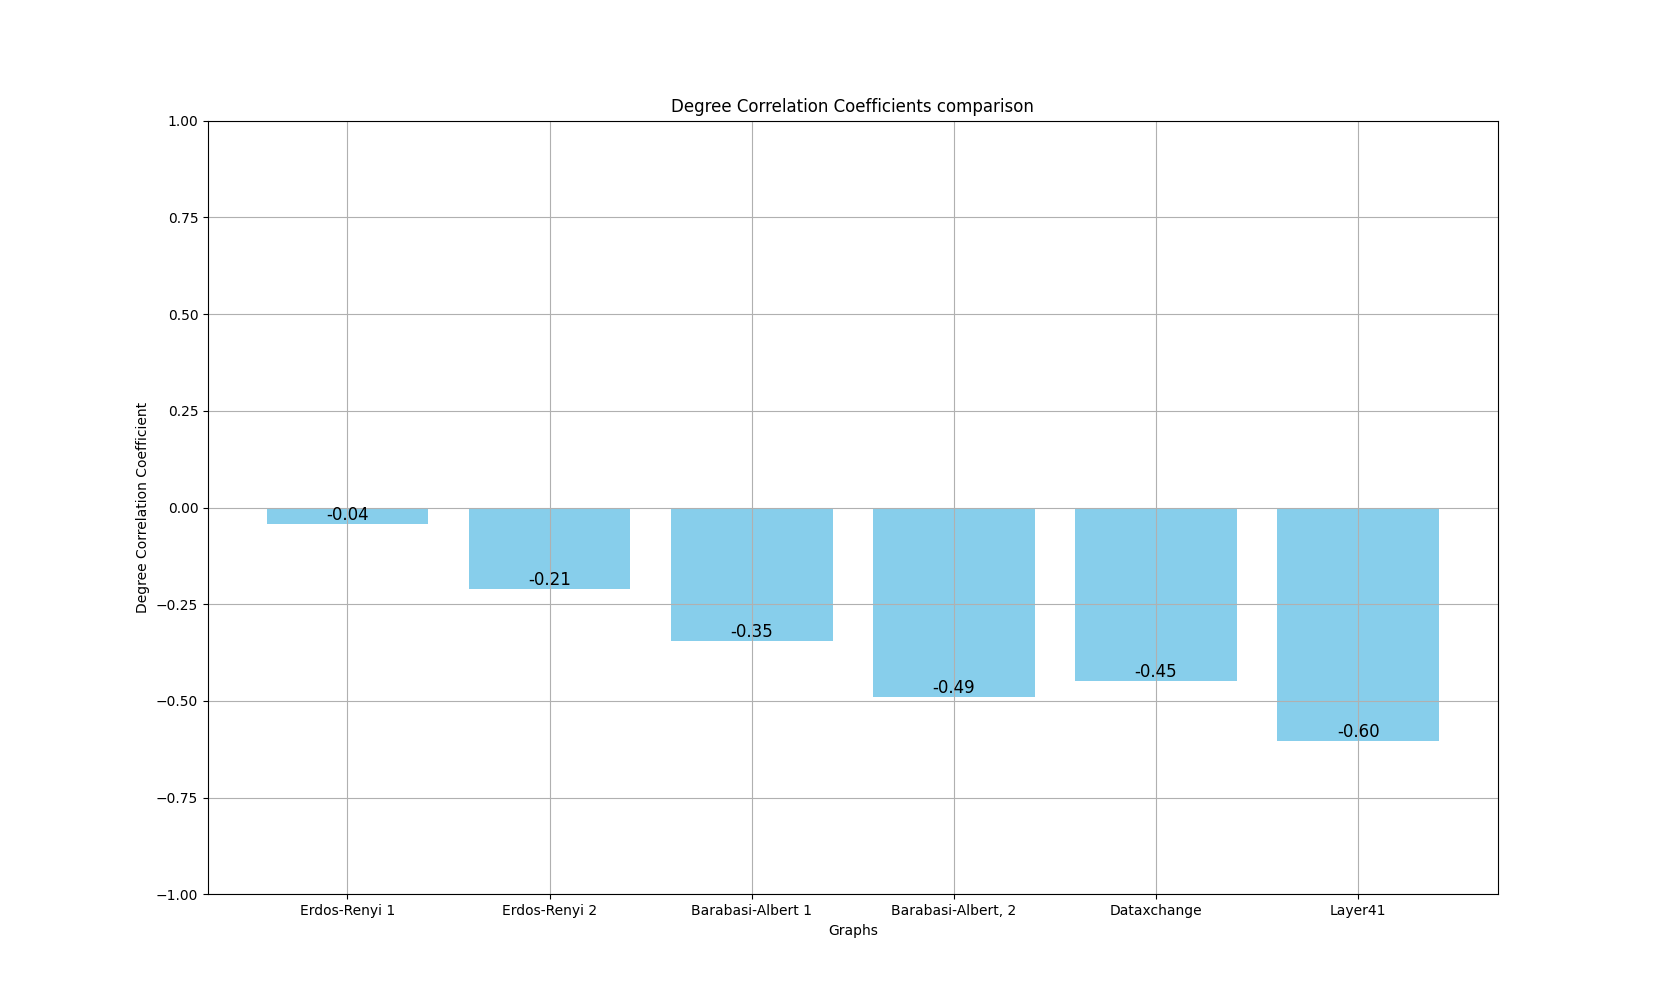
\includegraphics[width=0.9\linewidth]{images/FINAL-TOPO-COMP/Degree-correlation-coeff/deg-coeff-6.png}
    \caption{Degree correlation coefficient}
    \label{fig:enter-label}
\end{figure}

\subsubsection{Topology set 2}
Similarly to the previous topology set, the Erdos-Renyi graph generated using $p=0.3$, most closely matches both the Navigata and Nsfnet topologies with regards to shortest path length distribution. Particularly so with the Navigata topology.

\begin{figure}
    \centering
    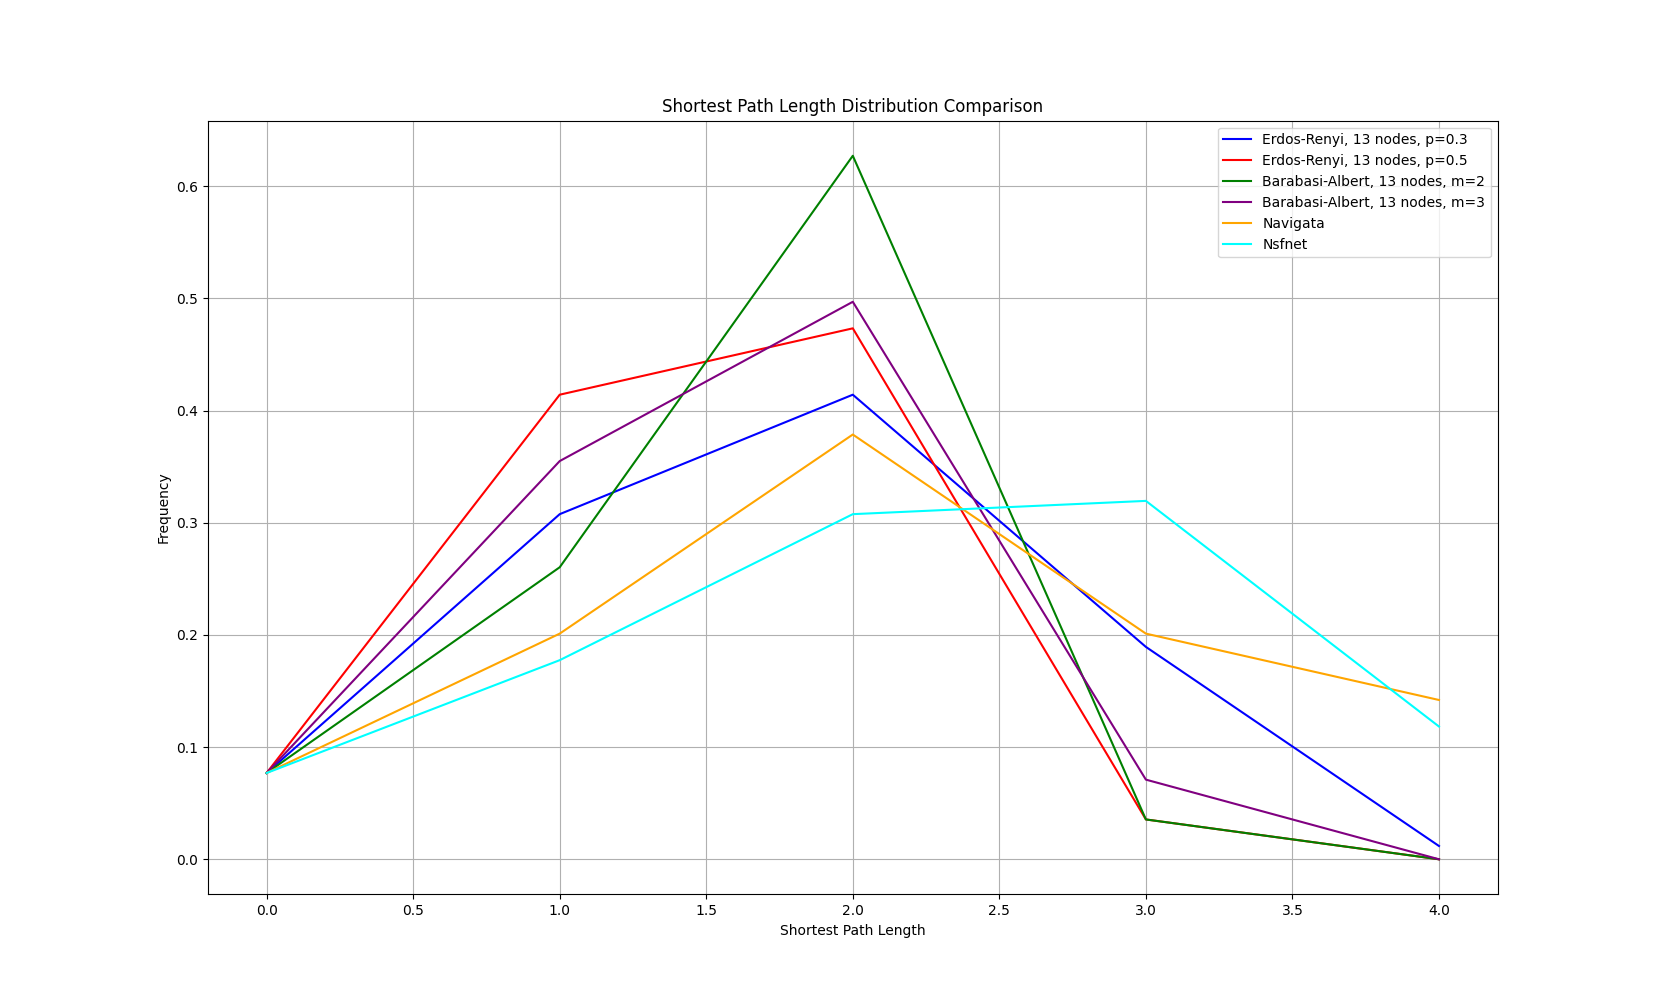
\includegraphics[width=0.9\linewidth]{images/FINAL-TOPO-COMP/line-13.png}
    \caption{Caption}
    \label{fig:enter-label}
\end{figure}

\begin{figure}
    \centering
    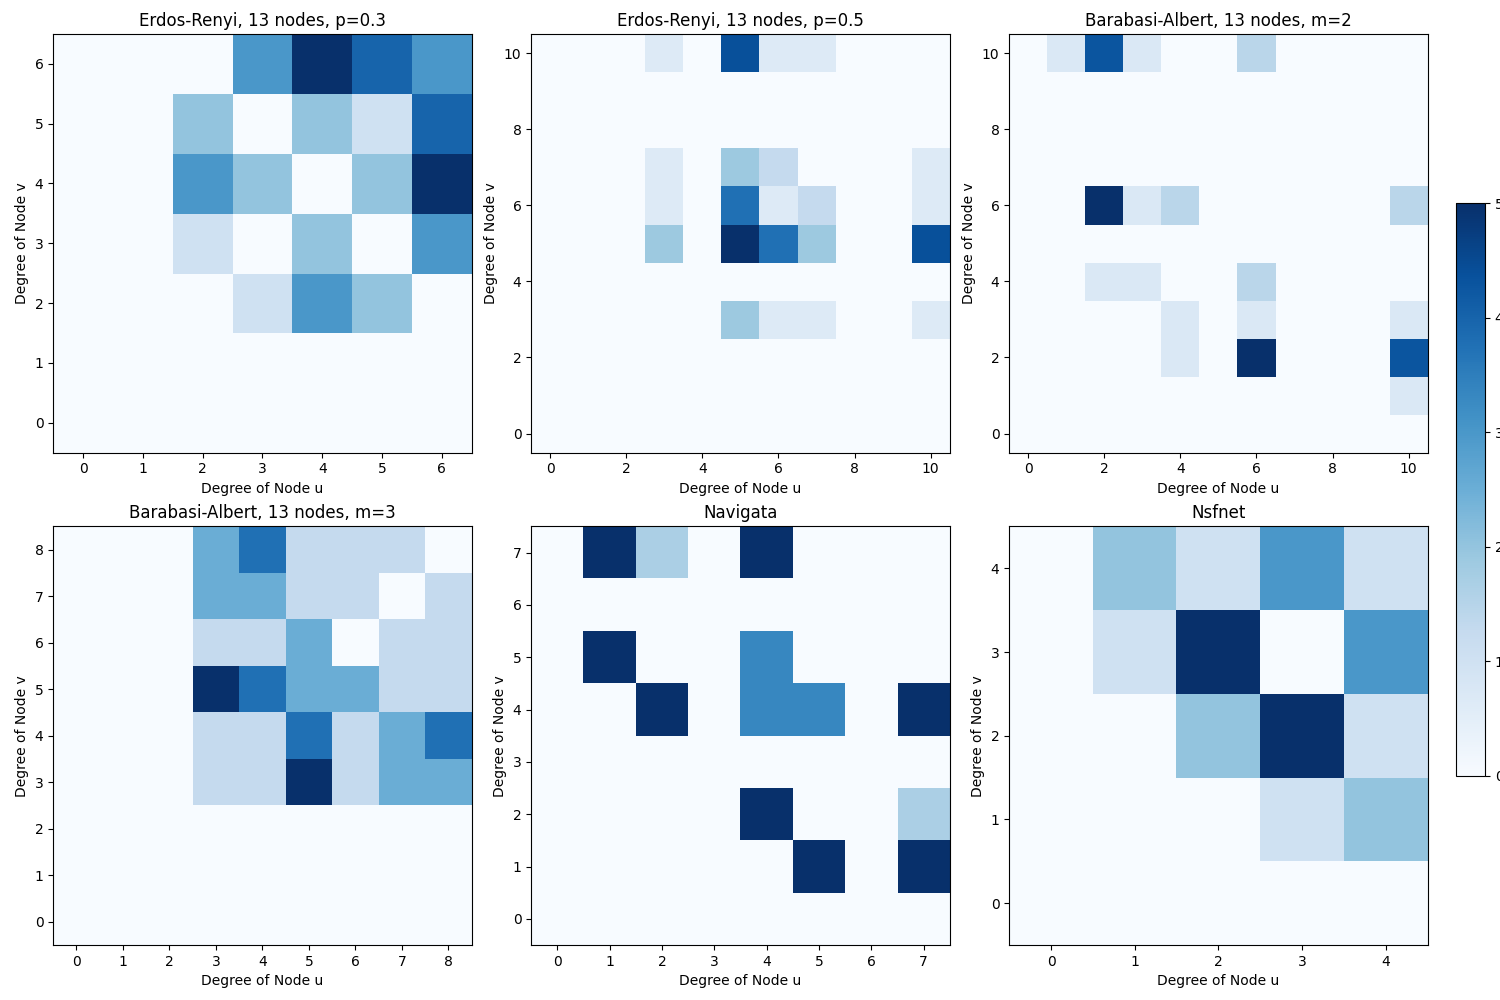
\includegraphics[width=0.9\linewidth]{images/FINAL-TOPO-COMP/Degree-correlation-matrices/13-matrix.png}
    \caption{Caption}
    \label{fig:enter-label}
\end{figure}

\begin{figure}
    \centering
    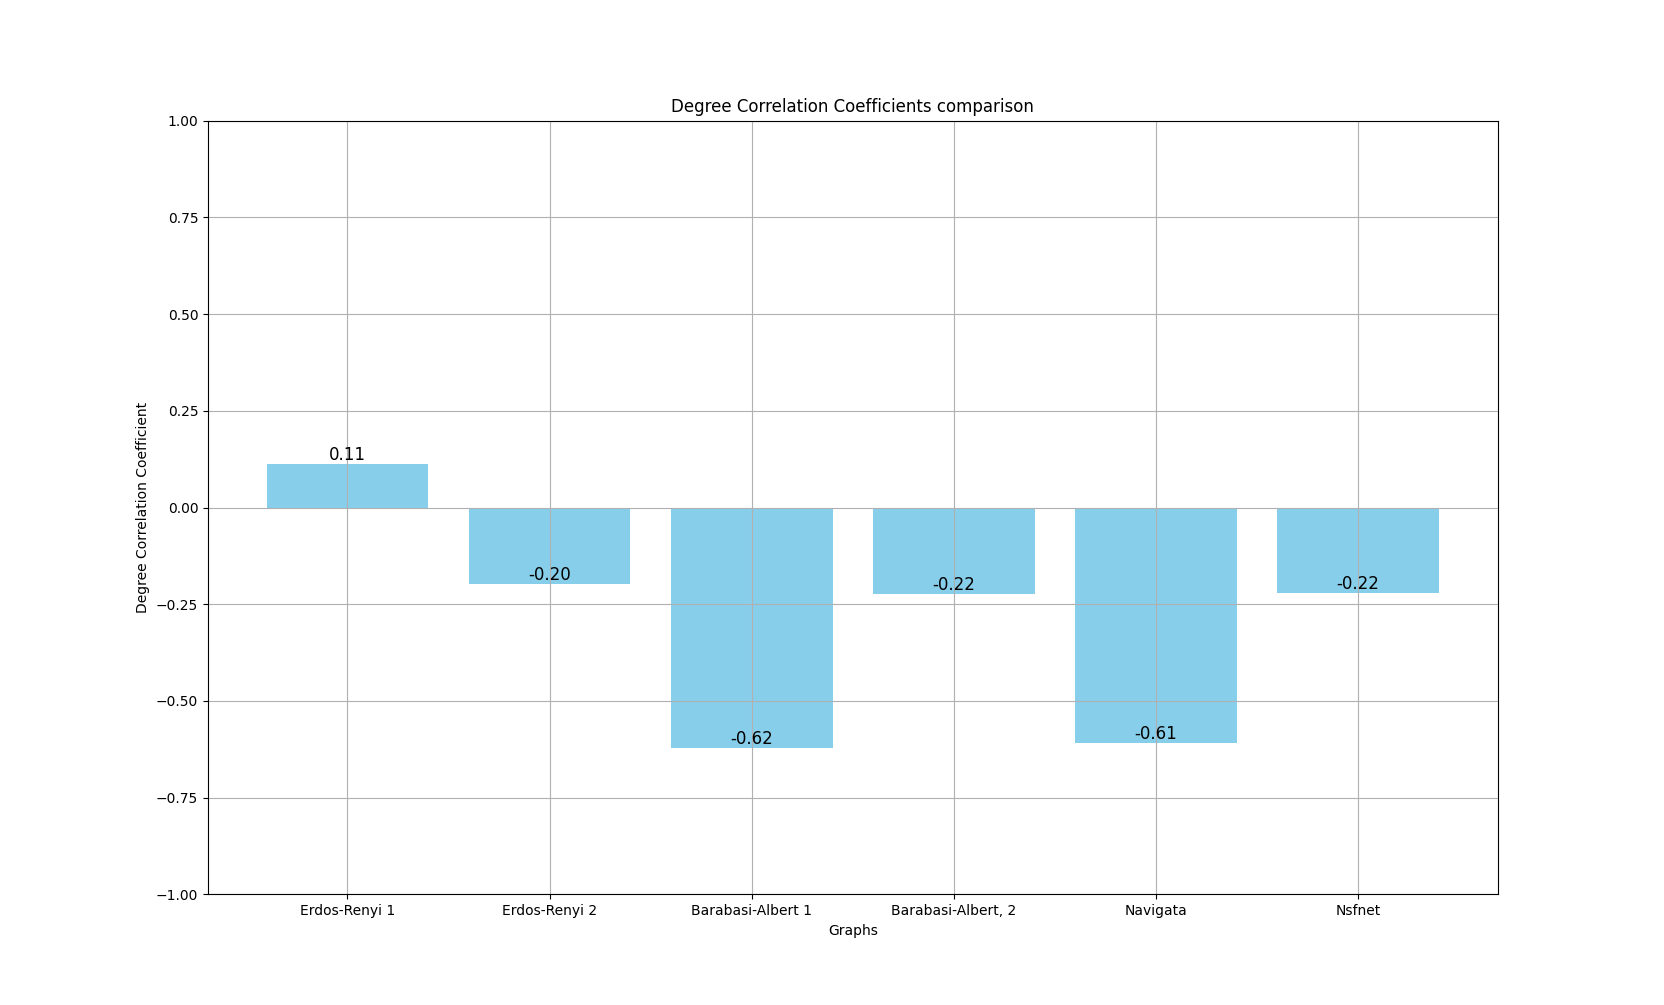
\includegraphics[width=0.9\linewidth]{images/FINAL-TOPO-COMP/Degree-correlation-coeff/deg-coeff-13.png}
    \caption{Degree correlation coefficient}
    \label{fig:enter-label}
\end{figure}

When comparing the degree correlation coefficient, both topologies generated using the Barabasi-Albert model match each of the real-world topologies respectively. With the m=2 model having a Degree correlation coefficent of -0.62, compared with Navigatas degree correlation coefficient of -0.61. Furthermore, the m=3 model has a degree correlation coefficient of -0.22 which is equal to Nsfnet's -0.22, additionally the Erdos-Renyi p=0.5 model is also close to Nsfnet with a degree correlation of -0.2. The Erdos-Renyi p=0.3 model has a positive degree correlation coefficient of 0.11, which categorises it as Dissasortative, the rest of the topologies have negative degree correlation coefficients categorising them as Assortative.

\subsection{Topology set 3}
None of the generated model's of size 20 nodes have a comparable Shortest path length distribution to either of the real-world models. The real-world topologies both have flatter shortest path length distribution profiles, peaking at approximately 0.3 frequency of a shortest path length 3. Contrastingly, the p=0.5 Erdos-Renyi generated topology rises sharply from 0 to peak at approximately 0.5 frequency for shortest path lengths 1 and 2, then sharply dropping back down to 0. Interestingly, the m=3 Barabasi-Albert model and p=0.3 Erdos-Renyi model have very similar Distribution profiles, peaking at approximately 0.6 frequency for a shortest path length of 2. 

\begin{figure}
    \centering
    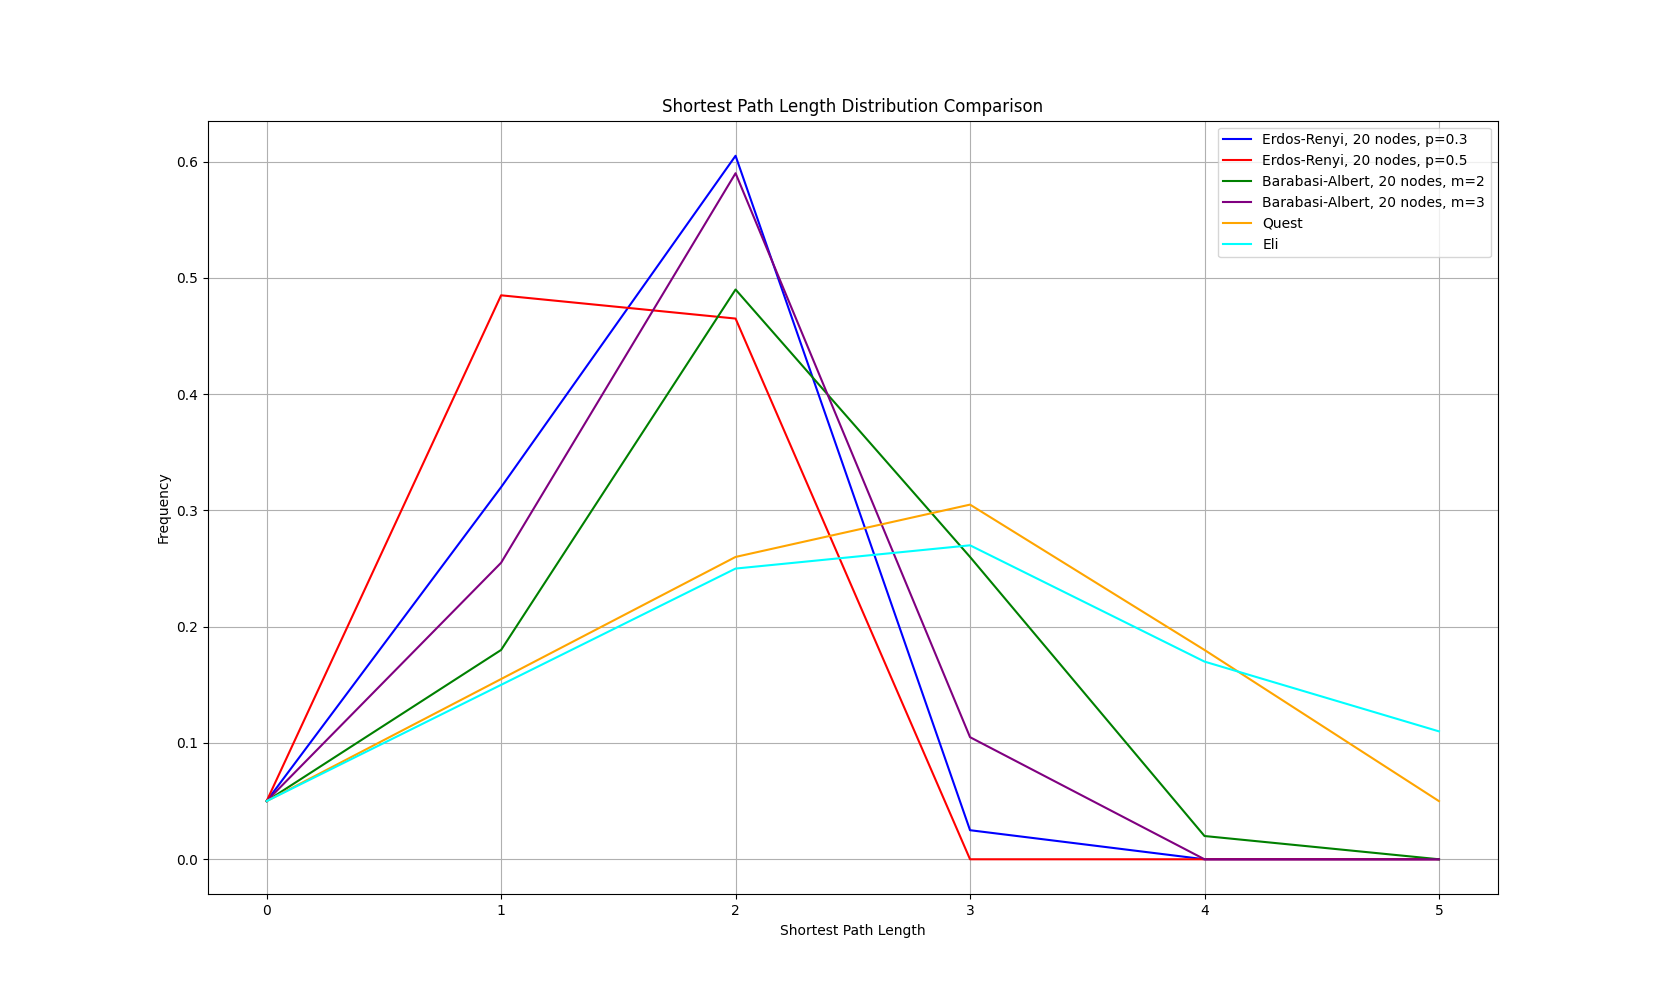
\includegraphics[width=0.9\linewidth]{images/FINAL-TOPO-COMP/line-20.png}
    \caption{Caption}
    \label{fig:enter-label}
\end{figure}

\begin{figure}
    \centering
    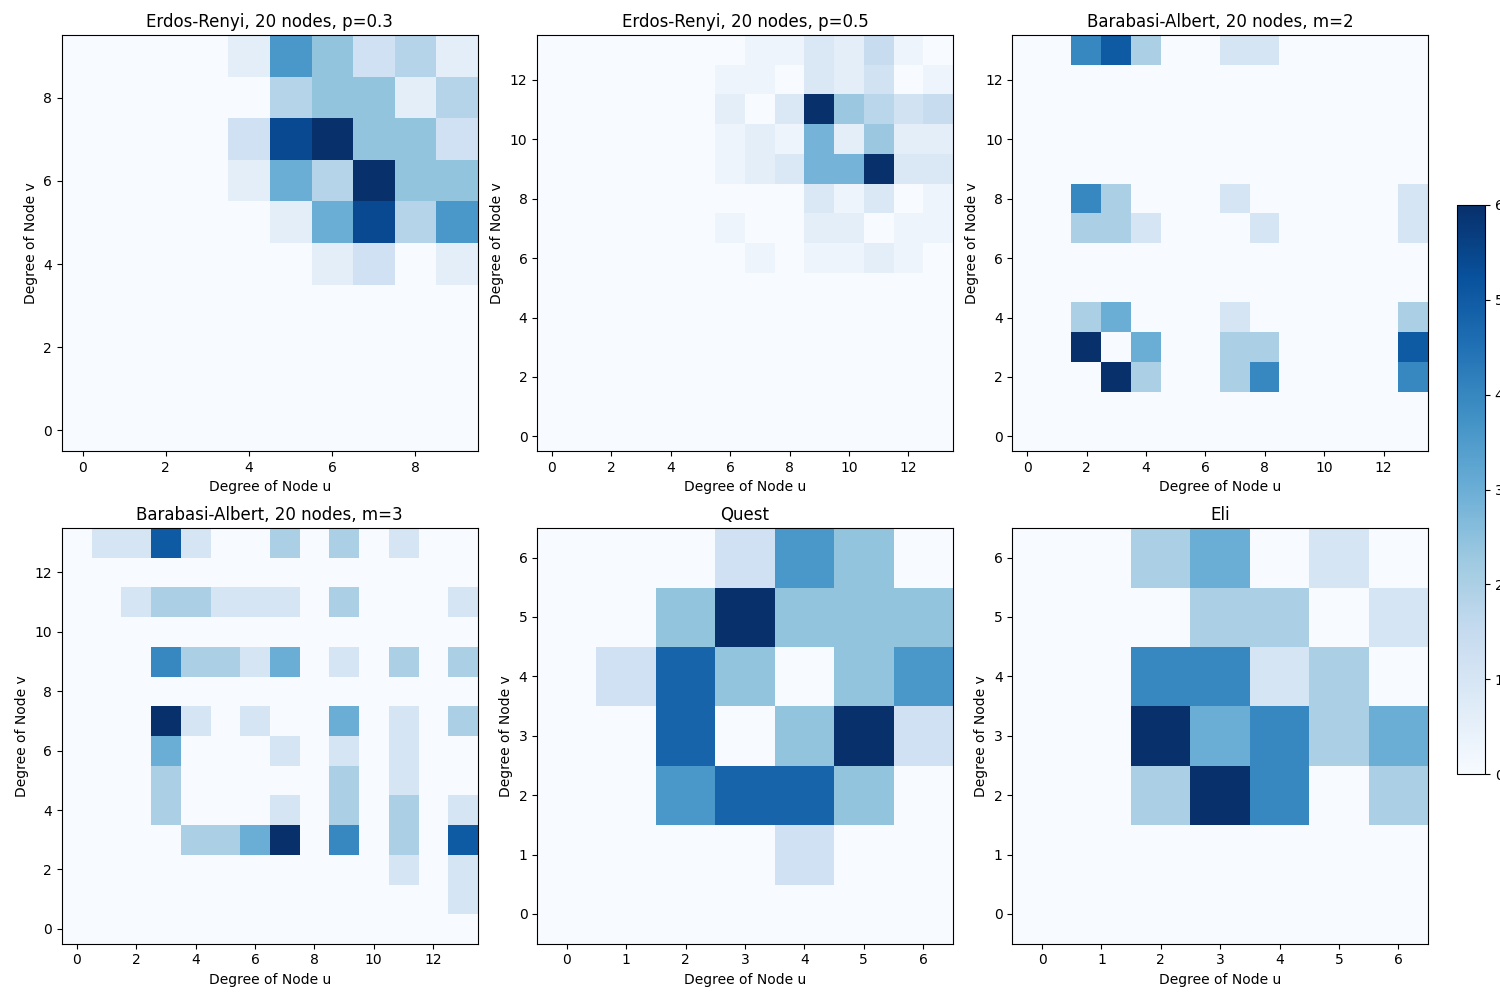
\includegraphics[width=0.9\linewidth]{images/FINAL-TOPO-COMP/Degree-correlation-matrices/20-matrix.png}
    \caption{Caption}
    \label{fig:enter-label}
\end{figure}

\begin{figure}
    \centering
    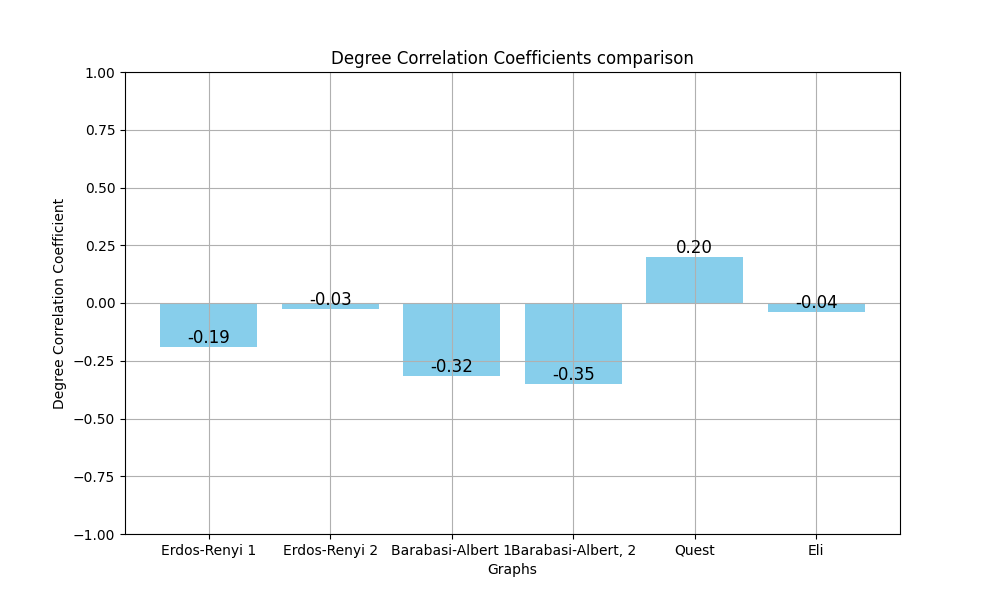
\includegraphics[width=0.9\linewidth]{images/FINAL-TOPO-COMP/Degree-correlation-coeff/deg-coeff-20.png}
    \caption{Degree correlation coefficient}
    \label{fig:enter-label}
\end{figure}
Through initial analysis of the varying degree correlation coefficients it is clear that the selected real-world topologies are distinct. With Quest having a positive degree correlation coefficient of 0.2 and Eli -0.04, this indicates that they are dissasortative and neutral topologies respectively. Out of the generated topologies the Erdos-Renyi p=0.5 model is similar to Eli, with a degree correlation coefficient of -0.03. 

\subsection{Topology set 4}
The shortest path length distribution of York, a real-world topology is relatively linear, maintaining a frequency of 0.3 shortest path lengths between 2 and 9. The generated topologies and Aconet have distinctly different profiles, with the Barabasi-Albert m=2 model having the closest shortest path length distribution to Aconet. Similarly to the previous topology set, the Erdos-Renyi p=0.3 and Barabasi-Albert m=3 model have very similar distributions, with both peaking just below 0.6 frequency for a shortest path length of 2. 

\begin{figure}
    \centering
    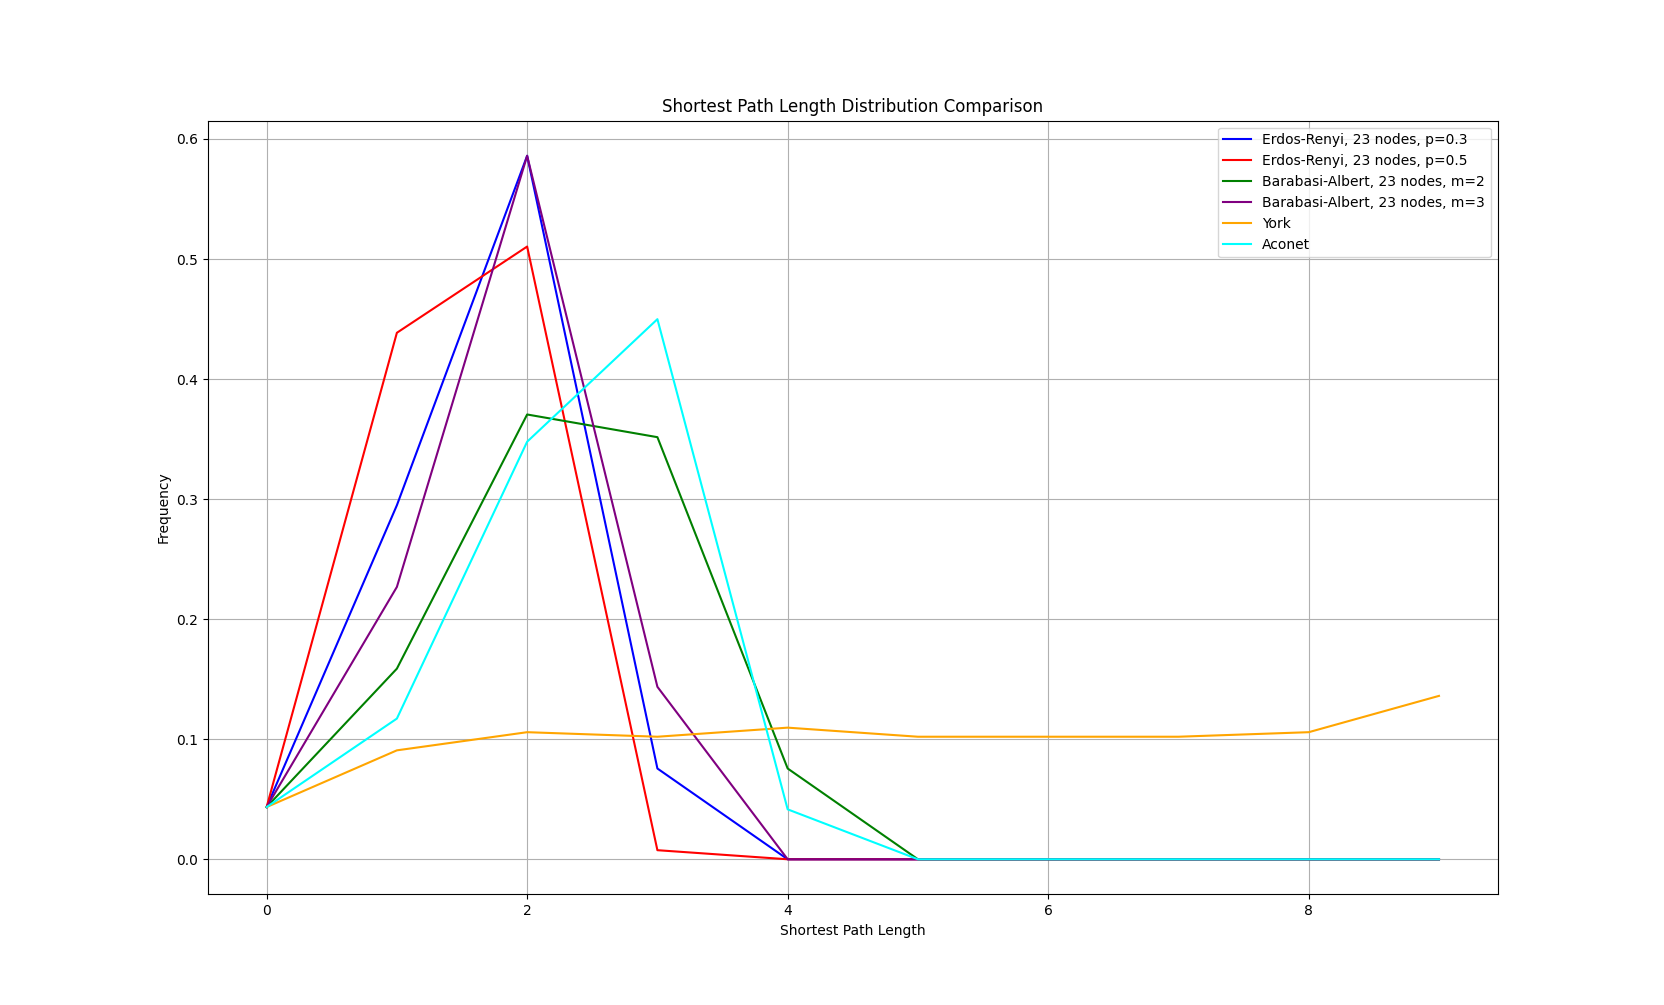
\includegraphics[width=0.9\linewidth]{images/FINAL-TOPO-COMP/line-23.png}
    \caption{Caption}
    \label{fig:enter-label}
\end{figure}

\begin{figure}
    \centering
    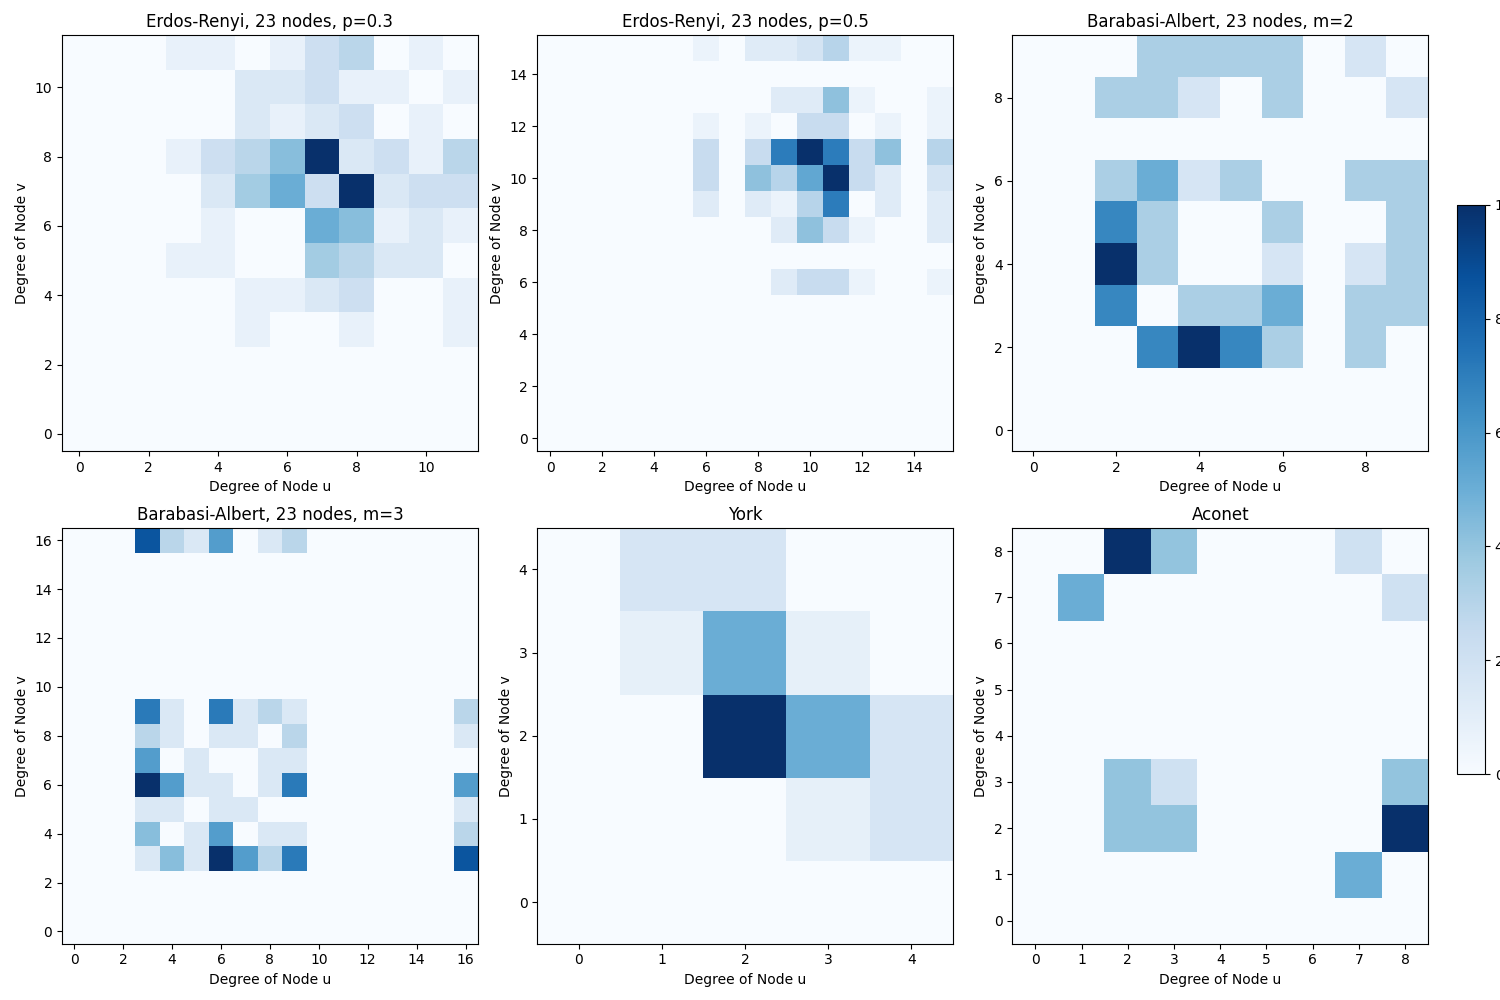
\includegraphics[width=0.9\linewidth]{images/FINAL-TOPO-COMP/Degree-correlation-matrices/23-matrix.png}
    \caption{Caption}
    \label{fig:enter-label}
\end{figure}
None of the four generated topologies have a similar degree correlation coefficient to the real-world topologies, with values ranging from -0.01 to -0.23 they are weakly assortative networks. However, the similarity is further established between the Erdos-Renyi p=0.3 and Barabasi-Albert m =3 models, both having comparible values of -0.12 and -0.23 respecitvely. Both York and Aconet are more strongly Assoratitive networks, with degree correlation coefficients of -0.51 and -0.4 respectively. 

\begin{figure}
    \centering
    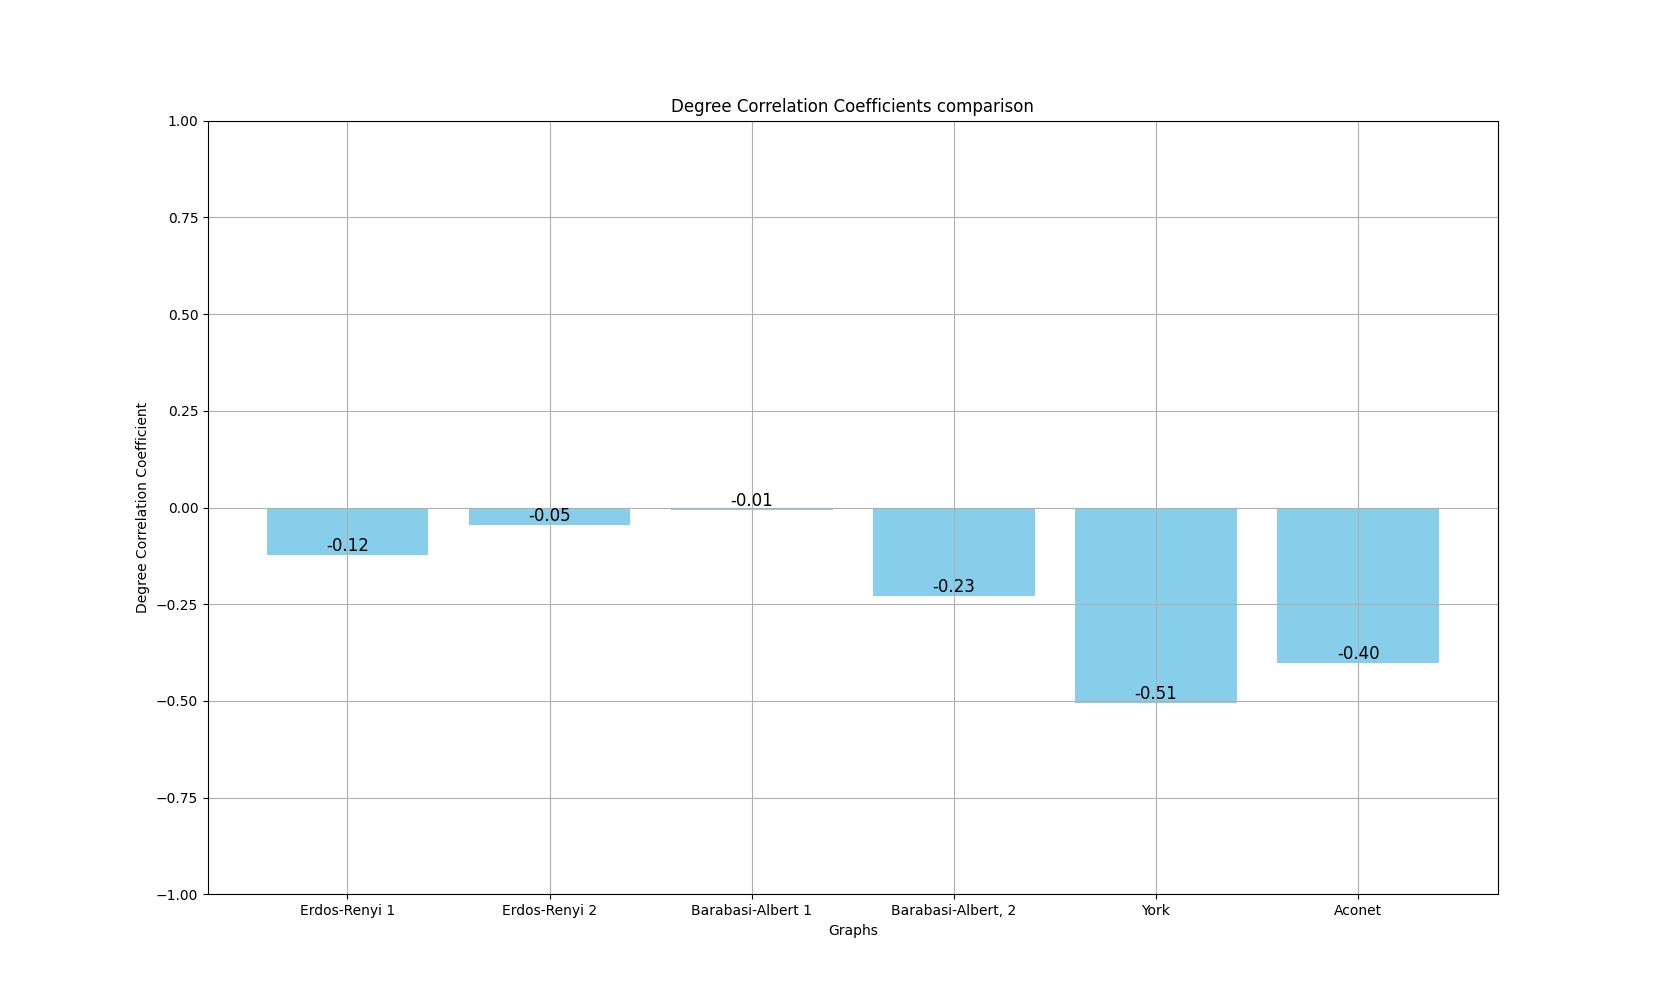
\includegraphics[width=0.9\linewidth]{images/FINAL-TOPO-COMP/Degree-correlation-coeff/deg-coeff-23.png}
    \caption{Degree correlation coefficient}
    \label{fig:enter-label}
\end{figure}

\subsection{Topology set 5}
Much like the previous topology set, the real-world topologies have a relatively flat profile. This might suggest a trend that increasing the network size flattens the shortest path length distribution. Additionally, also much like the previous topology sets the Erdos-Renyi p=0.3 and Barabasi-Albert m=3 topologies have very similar distributions. 
\begin{figure}
    \centering
    distribution 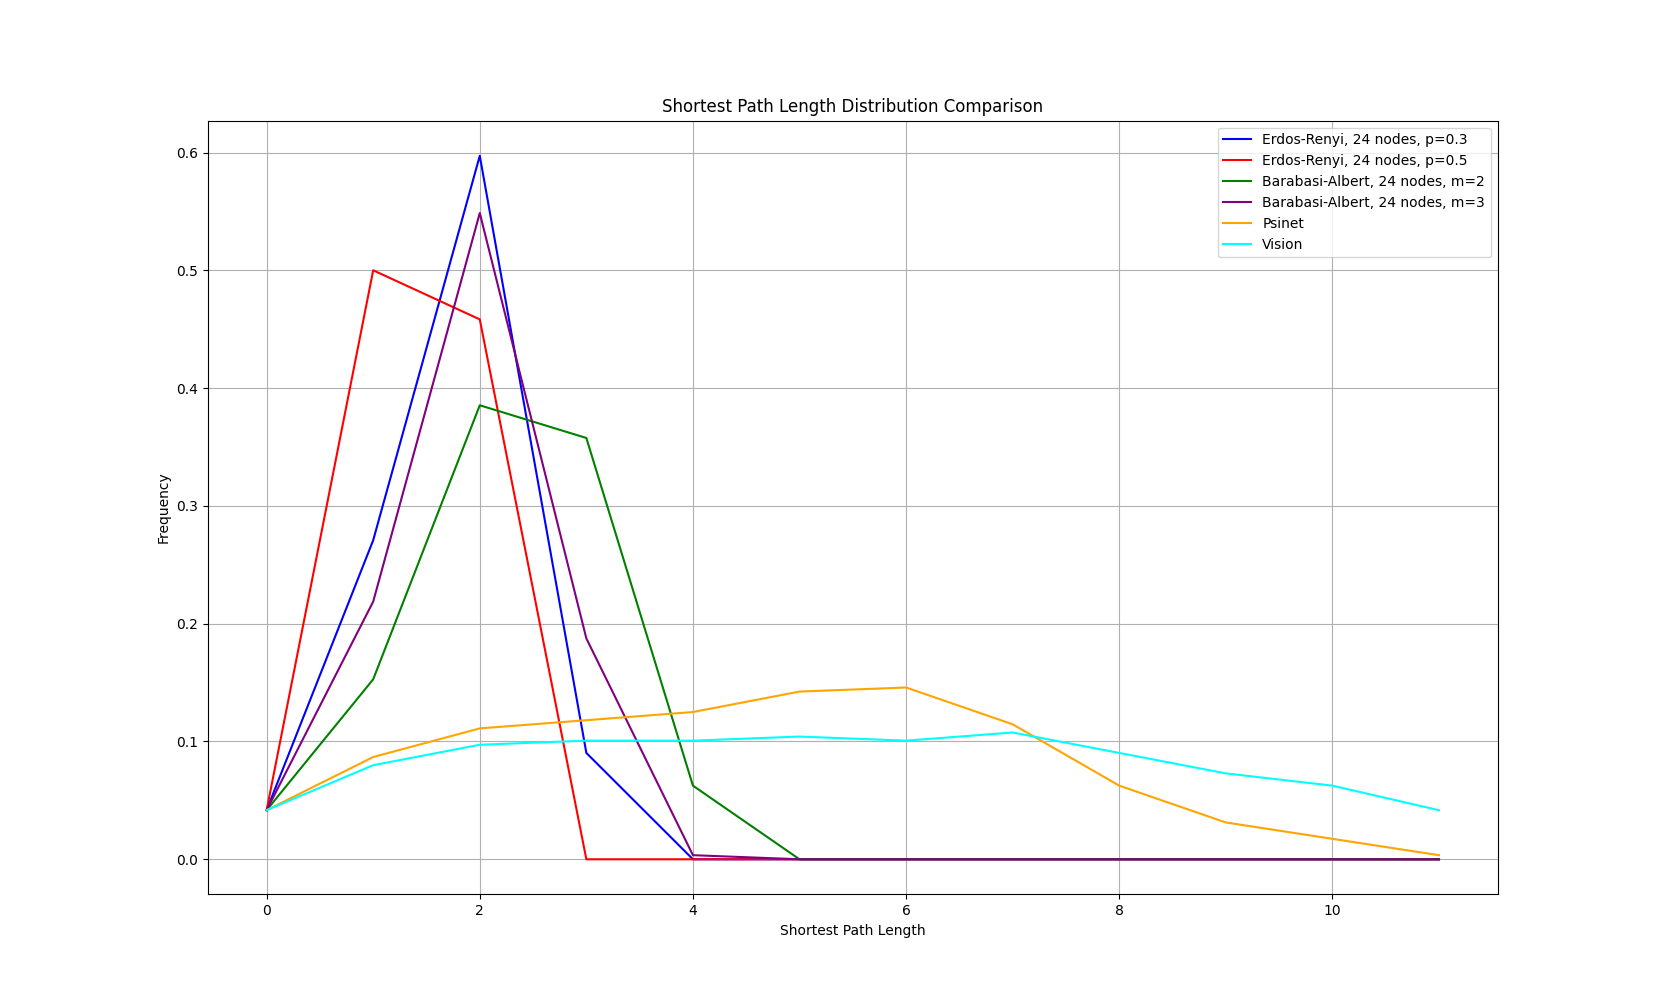
\includegraphics[width=0.9\linewidth]{images/FINAL-TOPO-COMP/line-24.png}
    \caption{Caption}
    \label{fig:enter-label}
\end{figure}

\begin{figure}
    \centering
    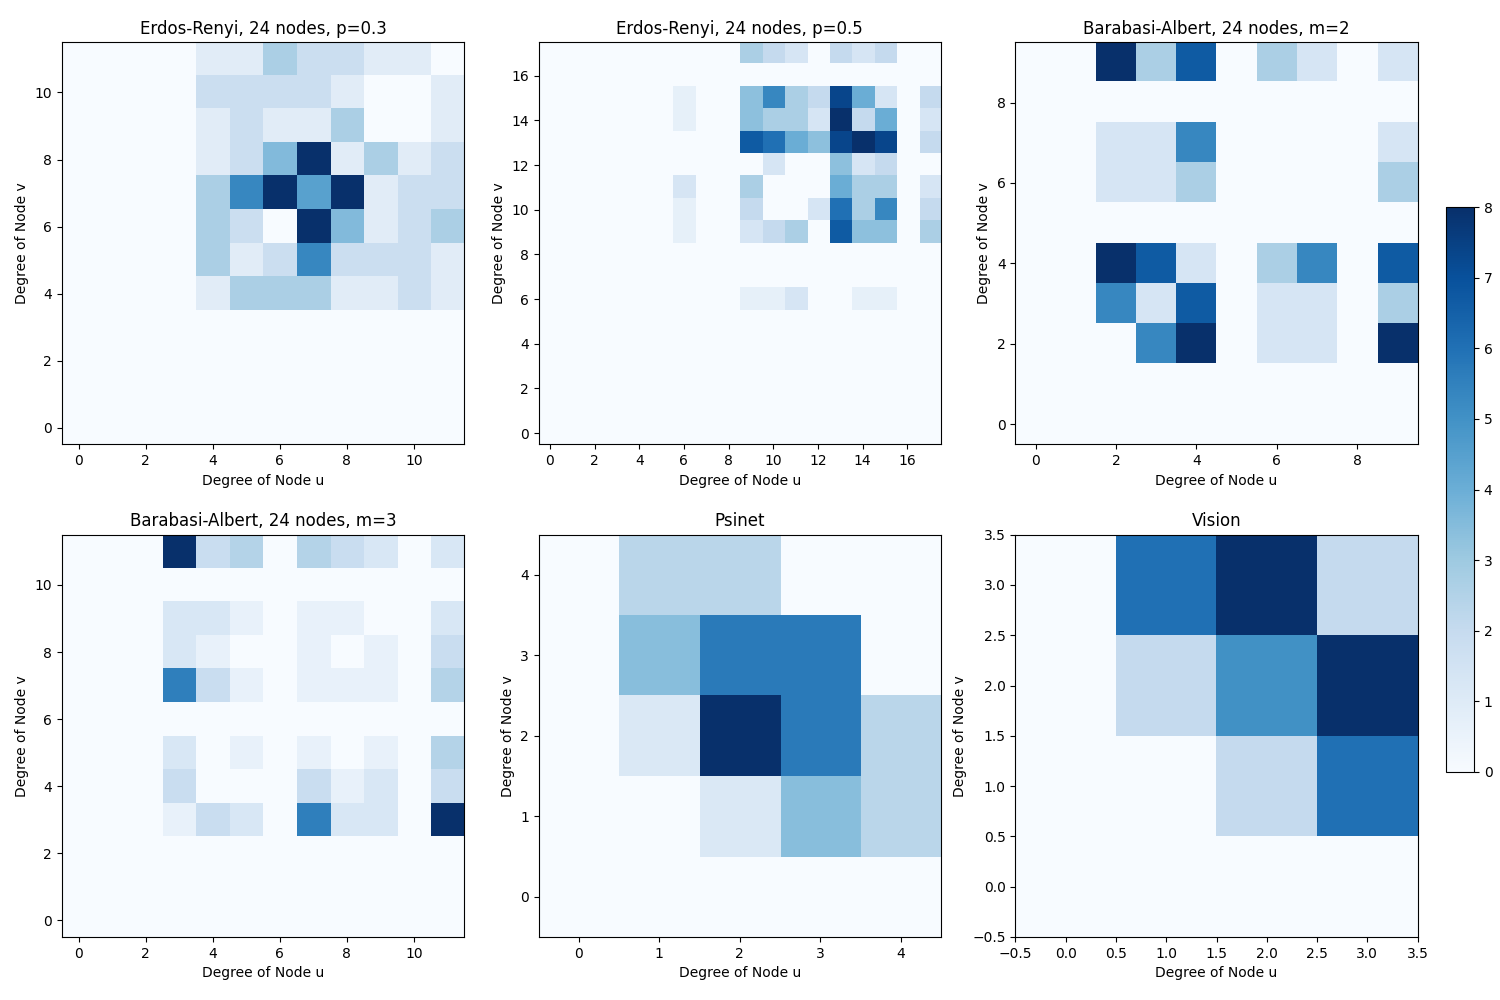
\includegraphics[width=0.9\linewidth]{images/FINAL-TOPO-COMP/Degree-correlation-matrices/24-matrix.png}
    \caption{Caption}
    \label{fig:enter-label}
\end{figure}

The comparison between the topology set shows an increasing degree correlation coefficient, with both the Erdos-Renyi models having values -0.05 and -0.10 which has some disparity with Psinet and Vision's degree corelation coefficient values of -0.37 and -0.43 respectively. Out of the generated topologies, only the Barabasi-Albert m=3 model is comparable to Psinet and vision, with a degree correlation coefficient of -0.37. 
\begin{figure}
    \centering
    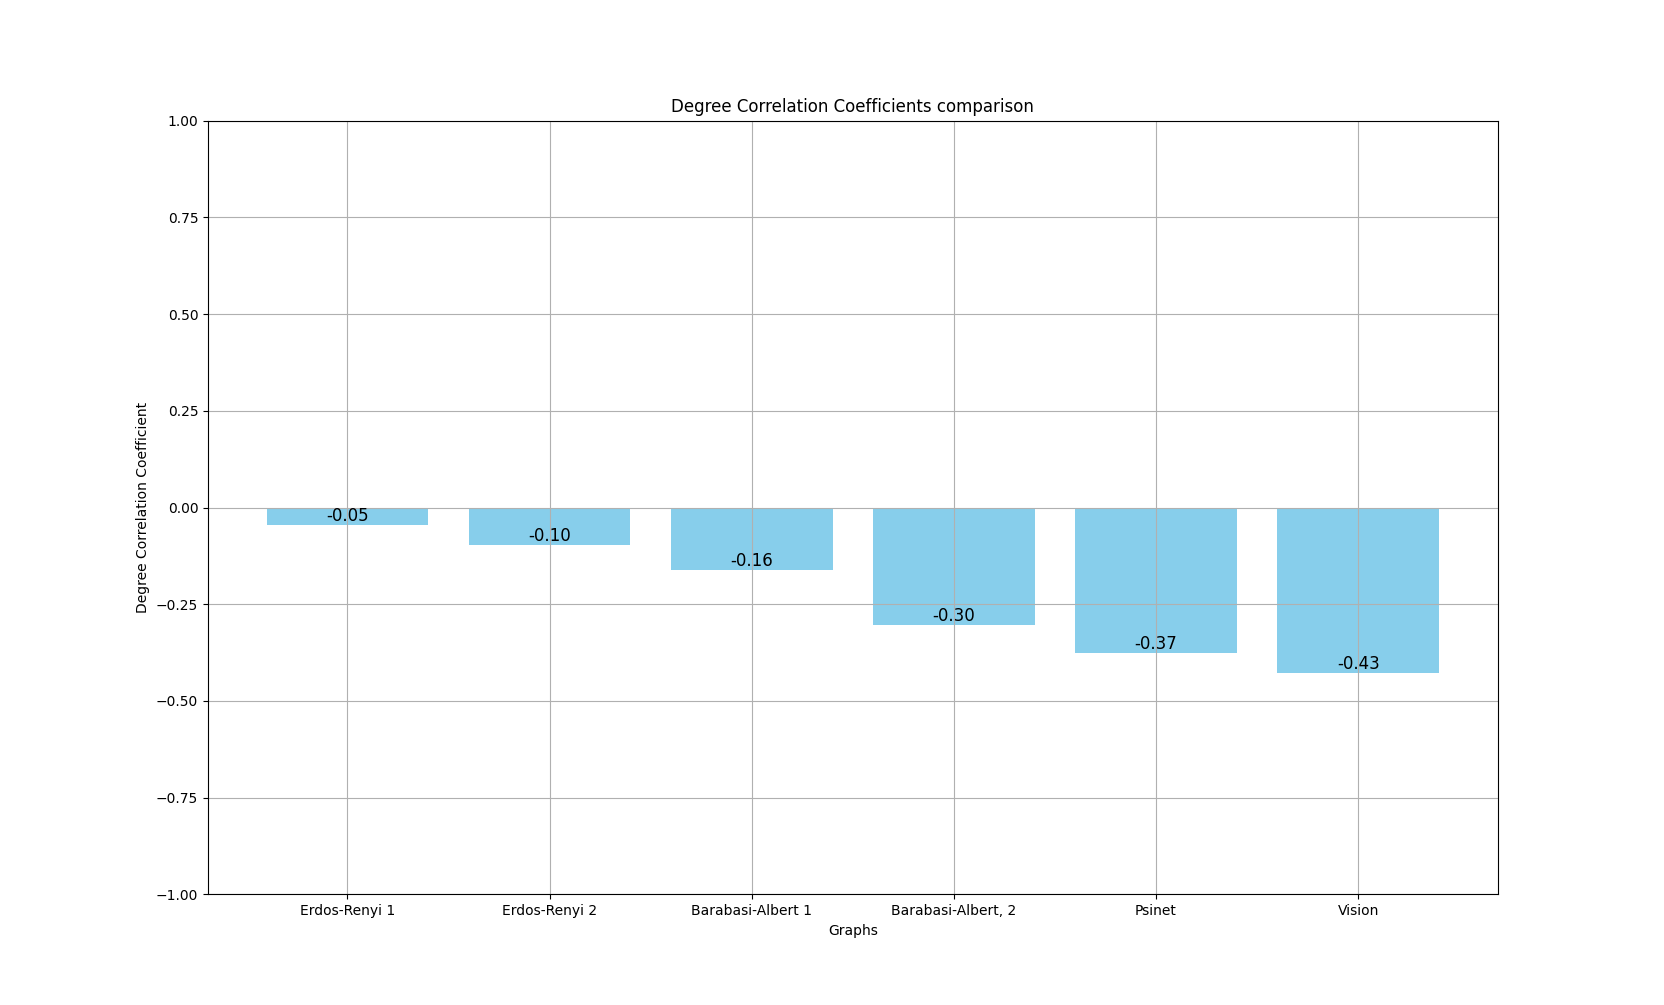
\includegraphics[width=0.9\linewidth]{images/FINAL-TOPO-COMP/Degree-correlation-coeff/deg-coeff-24.png}
    \caption{Degree correlation coefficient}
    \label{fig:enter-label}
\end{figure}

\subsection{Topology set 6}
Both Bbnplanet and Integra have very similar shortest path length distributions and a much flatter profile compared with the generated topologies; much like several of the previous real-world topologies. Furthermore, much like previous topology sets both the Erdos-Renyi p=0.3 model and Barabasi-Albert m=3 model have comparable distributions. 
\begin{figure}
    \centering
    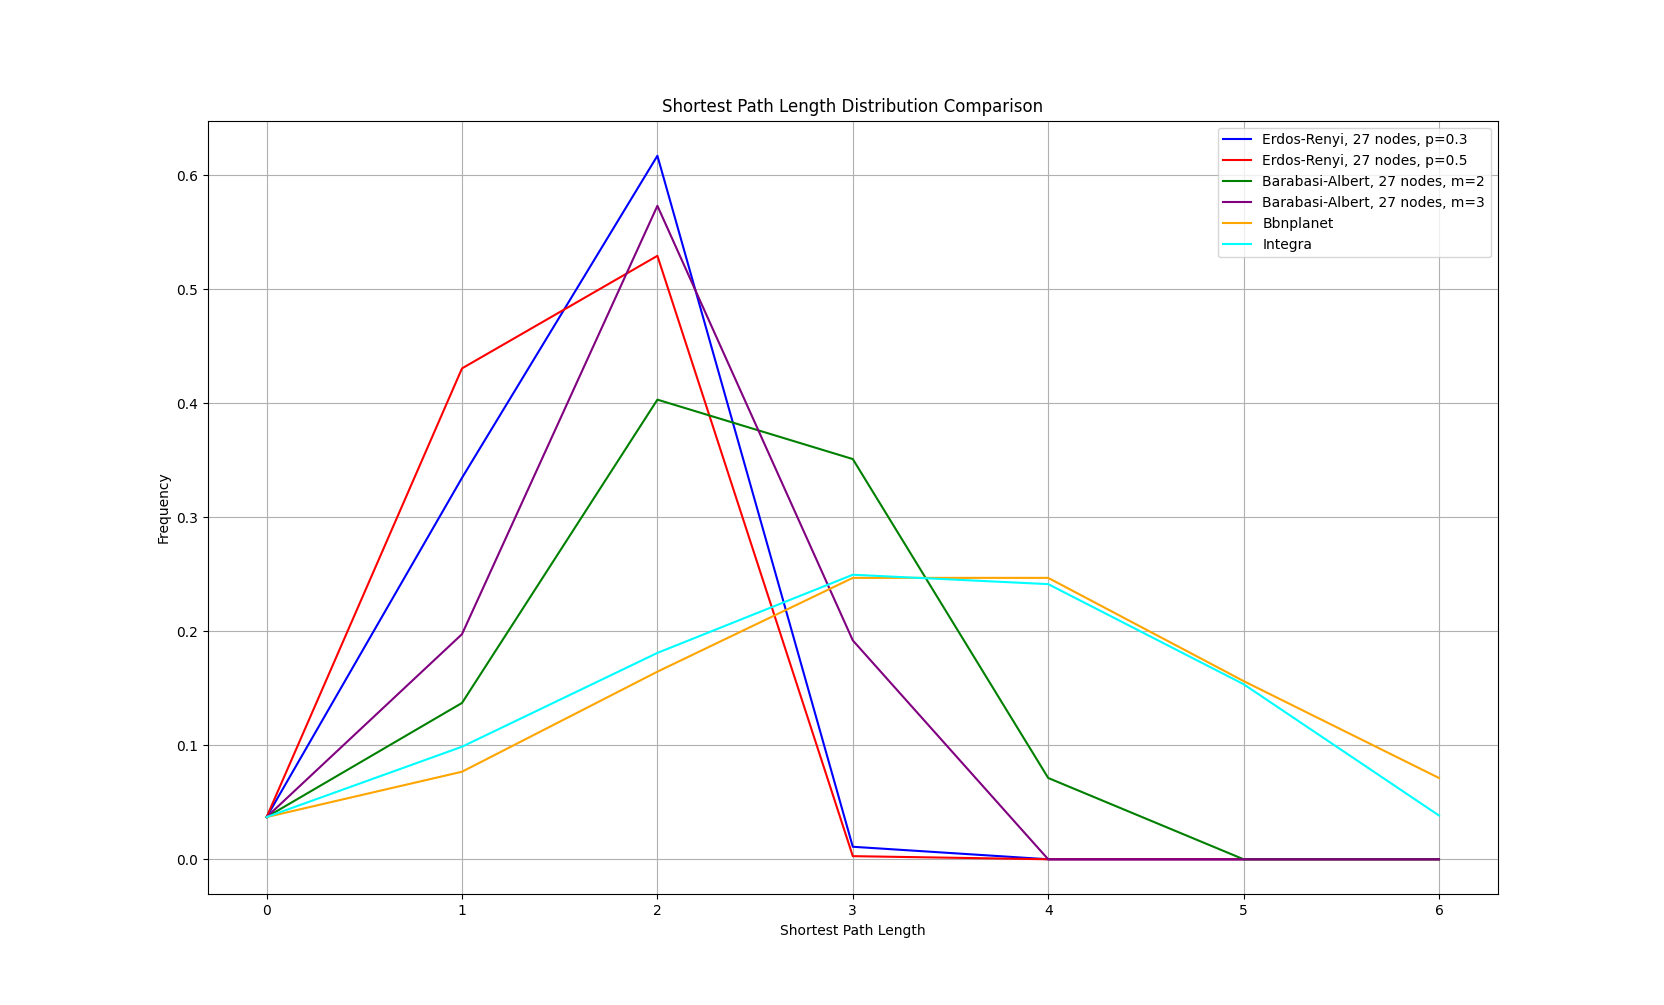
\includegraphics[width=0.9\linewidth]{images/FINAL-TOPO-COMP/line-27.png}
    \caption{Caption}
    \label{fig:enter-label}
\end{figure}

\begin{figure}
    \centering
    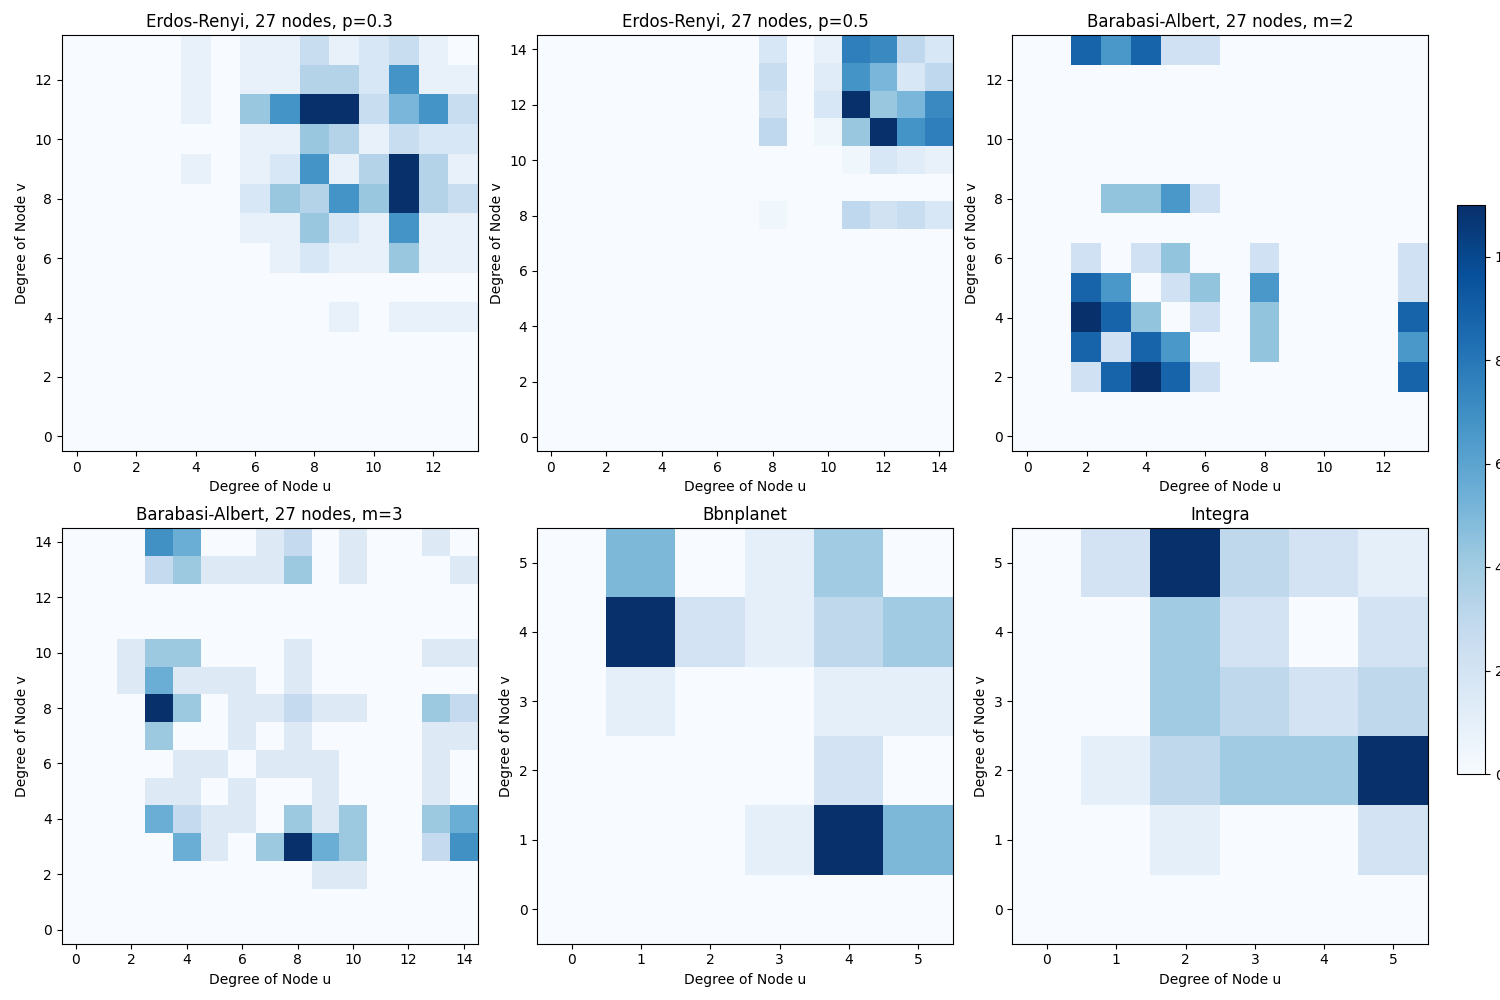
\includegraphics[width=0.9\linewidth]{images/FINAL-TOPO-COMP/Degree-correlation-matrices/27-matrix.png}
    \caption{Caption}
    \label{fig:enter-label}
\end{figure}

The degree correlation coefficient for both Erdos-Renyi generated topologies are slightly assoratitve, with $r$ values of -0.14 and -0.09 respectively. Additionally, both Barabasi-Albert models have lower degree correlation coefficient relative to the Erdos-Renyi with $r $values of -0.21 and -0.31 respectively. This echos previous results on the prior topology sets, whereby both types of generated models are generally assortative, with the Barabasi-Albert models having an elevated assortativity compared with the Erdos-Renyi models. 

\begin{figure}
    \centering
    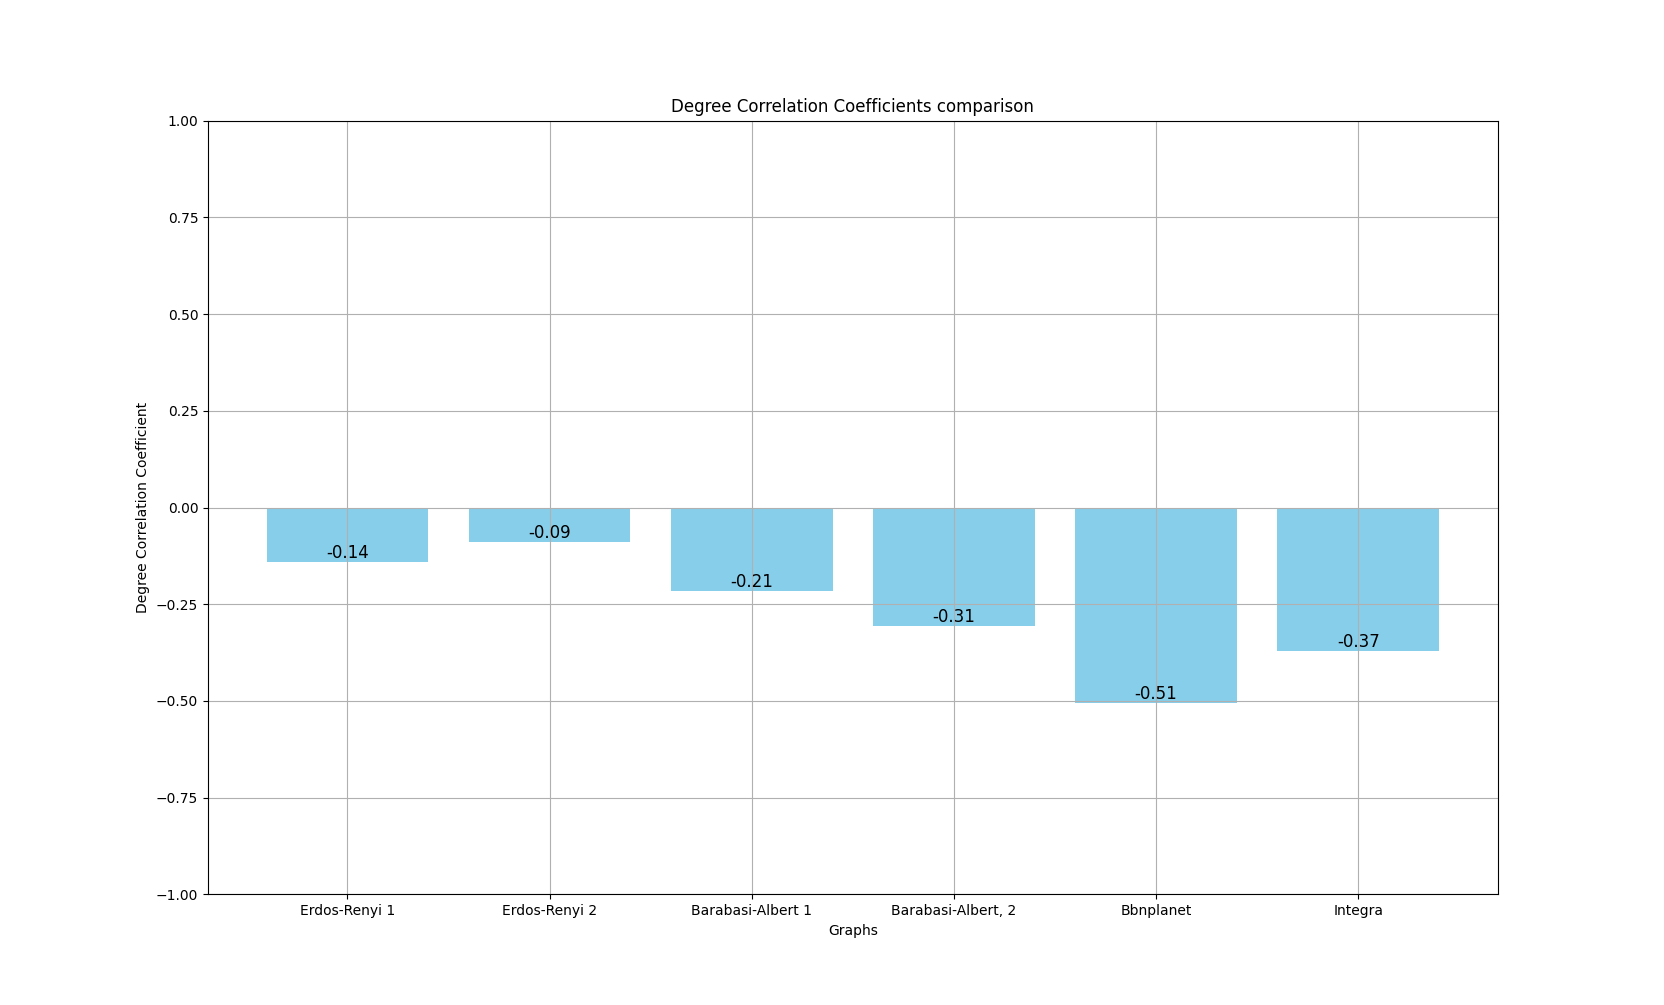
\includegraphics[width=0.9\linewidth]{images/FINAL-TOPO-COMP/Degree-correlation-coeff/deg-coeff-27.png}
    \caption{Degree correlation coefficient}
    \label{fig:enter-label}
\end{figure}

\subsection{Evaluation of Results}
Through evaluation of the comparison using statistical methods between the six sets of generated topologies and real-world topologies, clear trends are revealed. The mean degree correlation coefficient for every topology set was below -0.1, indicating that on average the topologies are assortative. The topology set with size 6 nodes has the lowest mean degree correlation coefficient of approximately -0.4, and the topology set of size 20 nodes has the highest mean degree correlation coefficient of approximately -0.1. The set comprising of topologies of size 13 nodes has the largest distribution.    

\begin{figure}
    \centering
    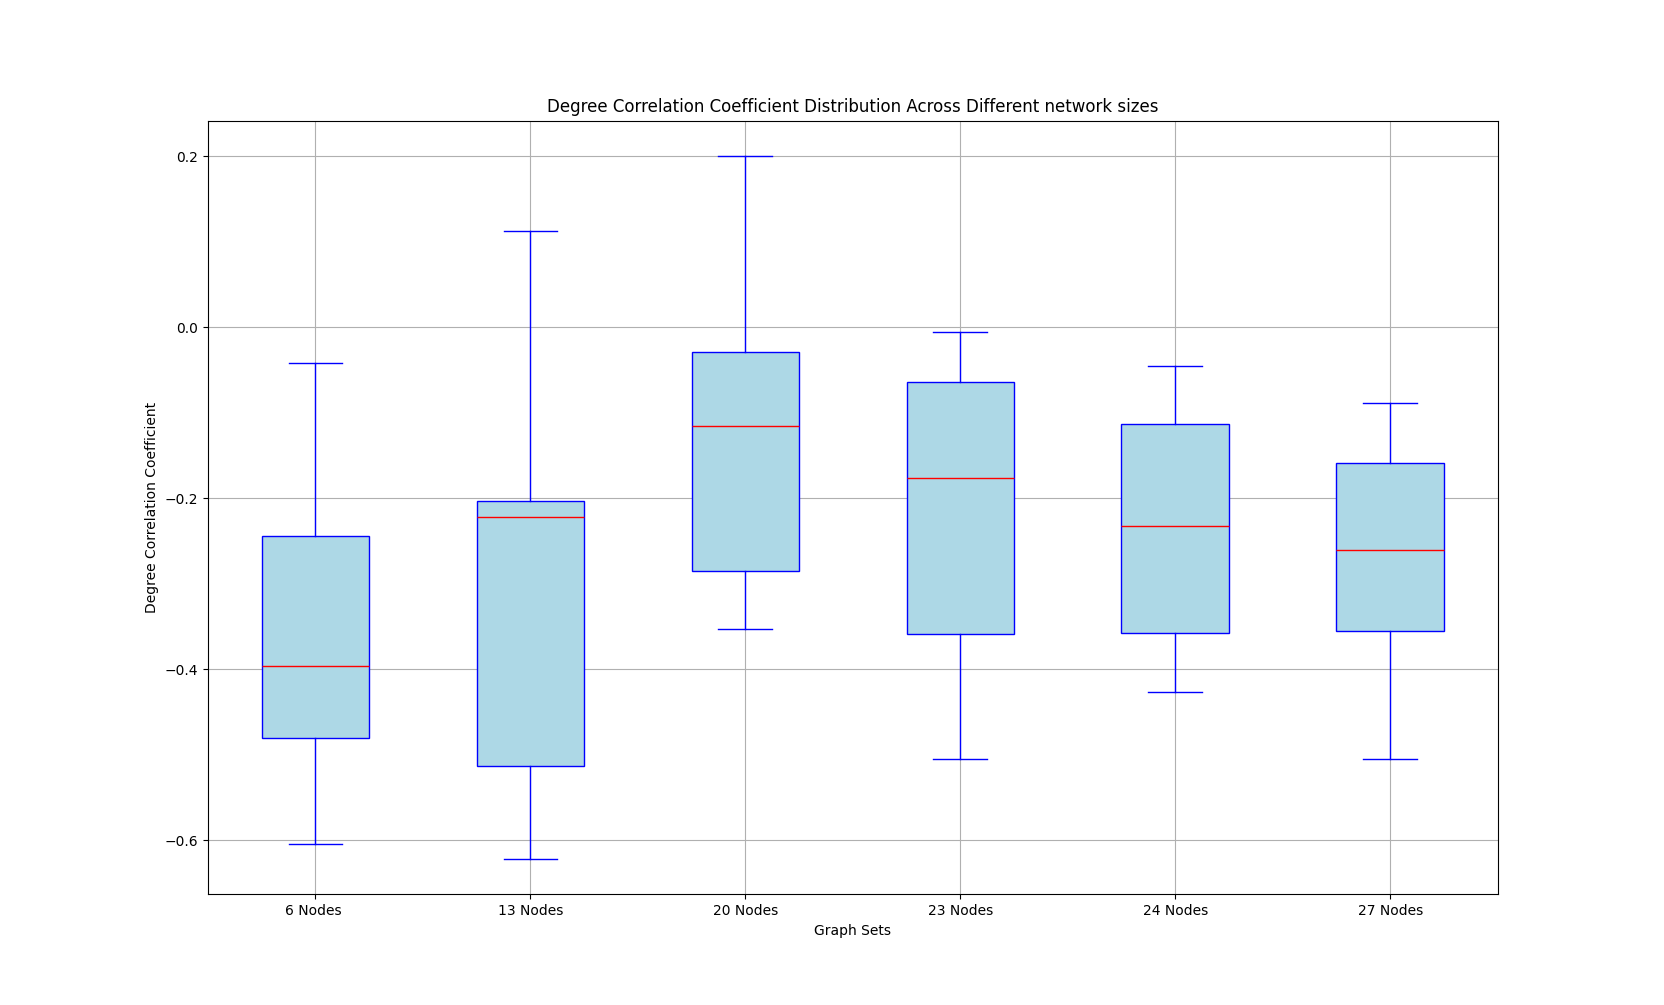
\includegraphics[width=0.9\linewidth]{images/FINAL-TOPO-COMP/Degree-coeff-distrib/Distrib-by-size.png}
    \caption{Caption}
    \label{fig:enter-label}
\end{figure}

The distribution plot below highlights that there is a distinct difference in degree correlation coefficient between each topology type. This range encompasses the Erdos-Renyi models, which are weakly assortative, the Barabasi-Albert models which are moderately assortative and the real-world models which are the most assortative. 

\begin{figure}
    \centering
    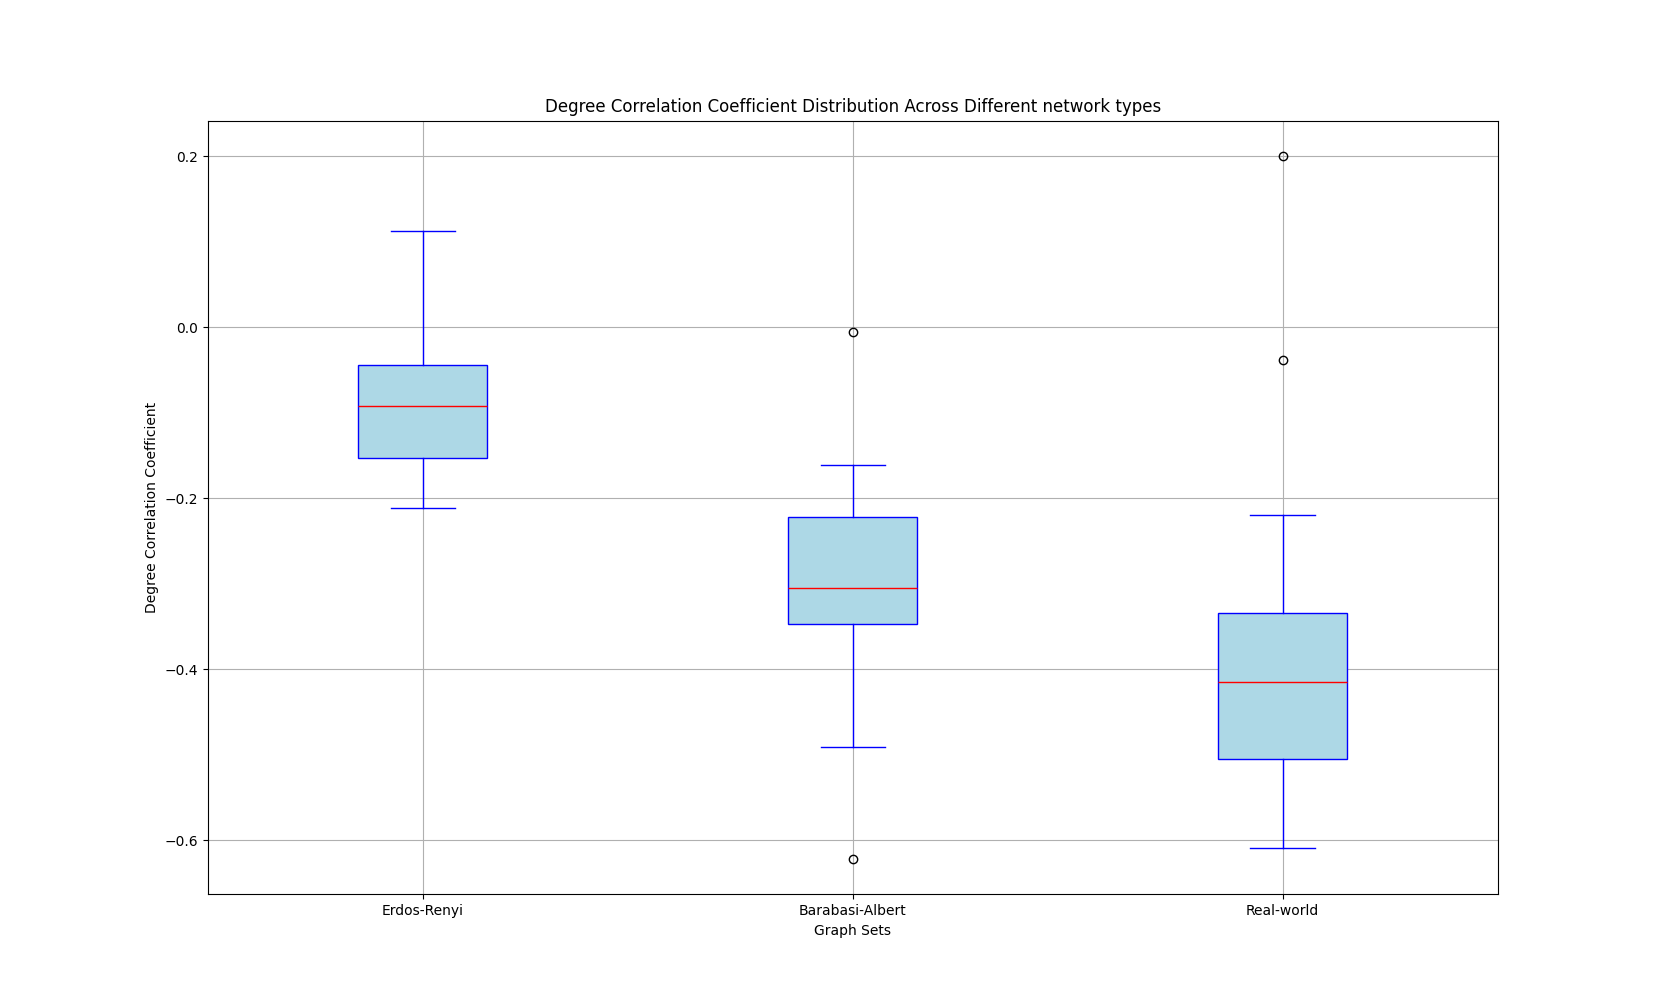
\includegraphics[width=0.9\linewidth]{images/FINAL-TOPO-COMP/Degree-coeff-distrib/Distrib-by-type.png}
    \caption{Caption}
    \label{fig:enter-label}
\end{figure}

\begin{figure}
    \centering
    \includegraphics[width=0.9\linewidth]{images/FINAL-TOPO-COMP/Degree-coeff-distrib/Distrib-by-param.png}
    \caption{Caption}
    \label{fig:enter-label}
\end{figure}

\begin{figure}
    \centering
    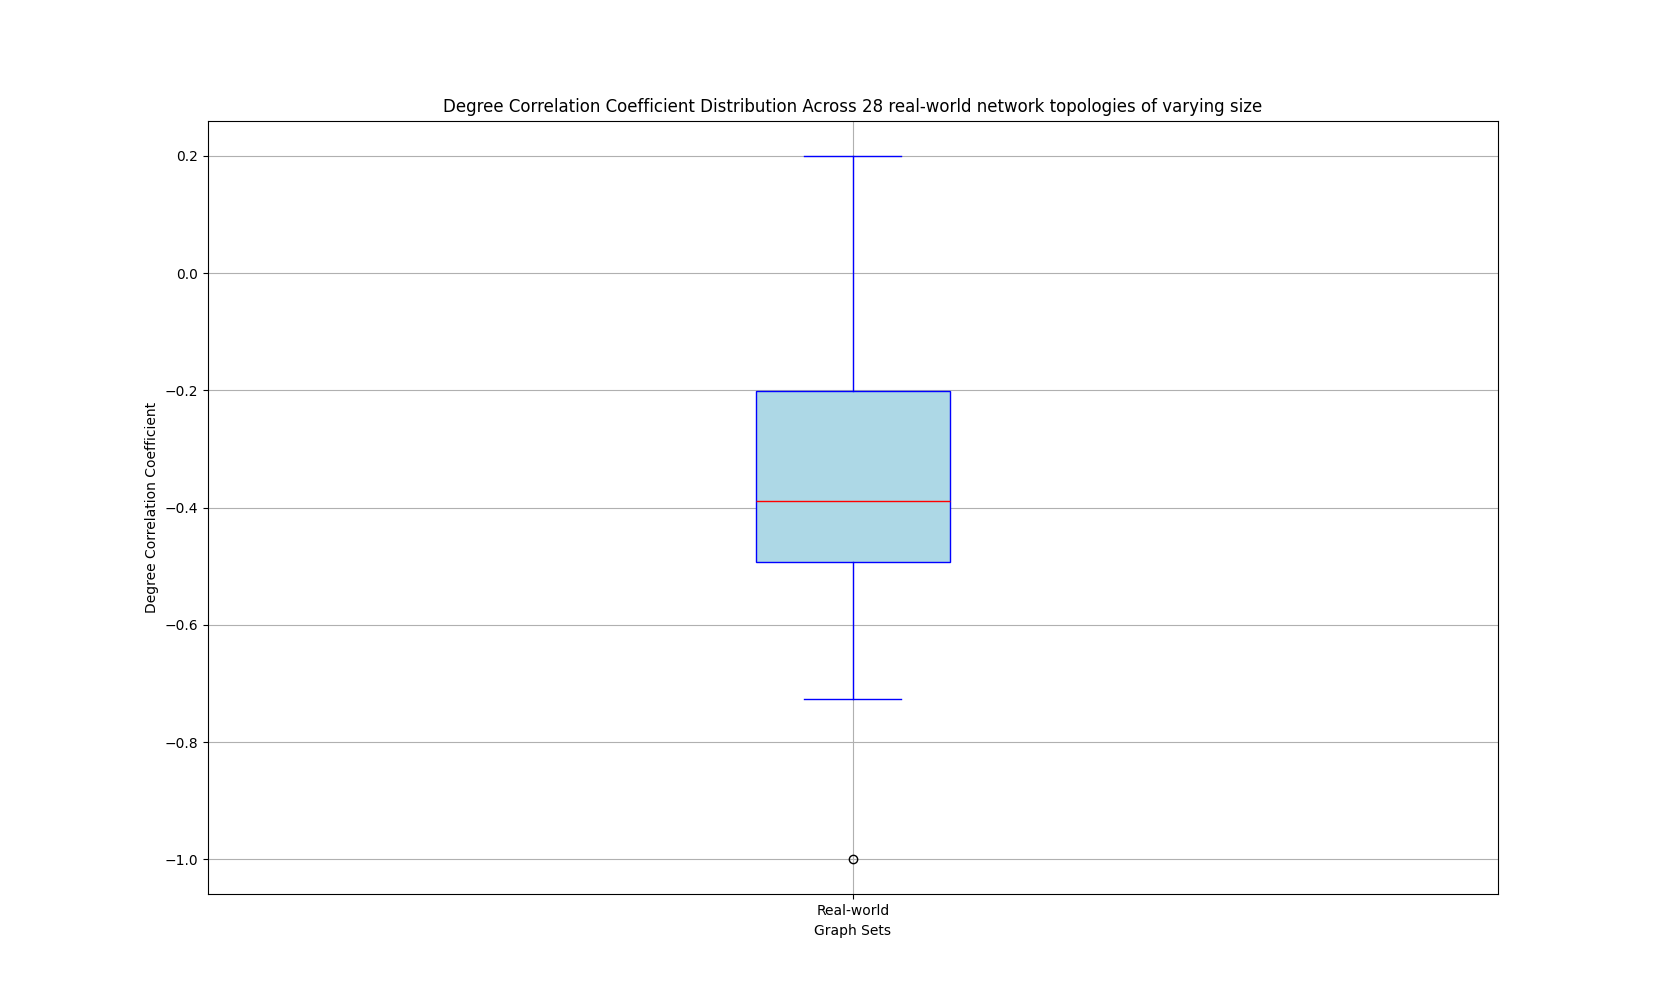
\includegraphics[width=0.9\linewidth]{images/FINAL-TOPO-COMP/Degree-coeff-distrib/Distrib-28-real-world.png}
    \caption{Caption}
    \label{fig:enter-label}
\end{figure}